\section{Dónde quedamos}
\label{sec:s11-donde-quedamos}

La Clase 10 definió los \(S\)-esquemas en la \cref{defi:s10-esquema-s}, las inmersiones cerradas en la \cref{defi:s10-inmersiones}, los puntos con valores en un cuerpo en la \cref{defi:s10-puntos-valores} y los morfismos afines, finitos y de tipo finito en la \cref{defi:s10-finitud}. Recordó el \cref{teo:s10-morfismos-destino-afin}, que identifica un morfismo de un esquema \(X\) a un afín \(\Spec A\) con un homomorfismo \(A\to\Gamma(X,\mathcal O_X)\), y demostró con él el \cref{lema:s10-morfismos-a-esquemas}, que dice lo mismo para morfismos de \(A\)-esquemas y homomorfismos de \(A\)-álgebras. Ese lema es la herramienta de hoy.

Con los \(K\)-puntos de la Clase 10, cada punto \(y\) de un esquema \(Y\) da el morfismo del punto \(i_y\colon\Spec\kappa(y)\to Y\) de la \cref{lema:s10-puntos-cuerpo-residual}(a), tomado con \(K=\kappa(y)\) e \(\iota=\id\). La 8d y la 9b calcularon a mano los primos de \(A[t]\) y de \(\mathbb Z[i]\) que están sobre un primo, en \cref{lema:s08-fibra-recta-afin,prop:s08-fibras-proyectiva,ejem:s09-enteros-gaussianos}. La 8a y la 8b construyeron \(\mathbb P_A^1\) por cartas para cualquier anillo \(A\), en la \cref{defi:s08-recta-proyectiva}. Hoy esas construcciones se comparan entre sí con una sola operación, el producto fibrado, y los cálculos a mano resultan ser el cálculo de una fibra. Lo que se usa está restablecido en la \cref{sec:s11-antecedentes} con su fuente.

\begin{obs}[Qué buscamos hoy]
\label{obs:s11-objetivos}
El producto fibrado de esquemas existe, y entre esquemas afines es el espectro del producto tensorial,
\[
 \Spec B\times_{\Spec A}\Spec C\cong\Spec(B\otimes_A C).
\]
Con él, el cambio de base de un esquema dado por ecuaciones con coeficientes en \(A\) a una \(A\)-álgebra \(B\) es el esquema de las mismas ecuaciones con coeficientes en \(B\), y la recta proyectiva cumple
\[
 \mathbb P_{\mathbb Z}^1\times_{\Spec\mathbb Z}\Spec\mathbb F_p\cong\mathbb P_{\mathbb F_p}^1
\]
por el \cref{lema:s11-proyectiva-fp}, cuyo esbozo es de lectura. La fibra de un morfismo \(f\colon X\to Y\) sobre un punto \(y\) es el cambio de base \(X_y=X\times_Y\Spec\kappa(y)\), un \(\kappa(y)\)-esquema cuyo espacio es la preimagen \(f^{-1}(y)\). En el caso afín, sus puntos son los primos de \(B\) que contraen a \(\mathfrak p\), que es lo que se calculó a mano.

El ejemplo nuevo es la familia \(T_1T_2^2=m\) sobre \(\Spec\mathbb Z\), integral, con fibras que tienen nilpotentes sobre los primos que dividen a \(m\). Las fibras de \(\Spec\mathbb Z[i]\), de la familia \(xy=n\) y de \(\mathbb P^1_{\mathbb Z}\), ya vistas, quedan de lectura. El ejemplo \(\mathbb C\otimes_{\mathbb R}\mathbb C\cong\mathbb C\times\mathbb C\), de lectura, muestra que el espacio de un producto fibrado puede tener más puntos que el producto fibrado de los conjuntos, y en la fibra los dos coinciden por el \cref{teo:s11-espacio-fibra}.
\end{obs}

\section{Lo que se usa hoy}
\label{sec:s11-antecedentes}

Todo anillo es conmutativo y con unidad, y todo homomorfismo de anillos lleva \(1\) en \(1\). Las referencias a Vakil son a \emph{The Rising Sea}, borrador del 21 de octubre de 2025, y las de Liu a \emph{Algebraic Geometry and Arithmetic Curves} (Oxford, 2002). Los resultados de las clases anteriores se restablecen con su enunciado y su fuente, y su demostración está en las notas de esa clase. La \cref{prop:s11-polinomios-tensorial} y la parte con polinomios de la \cref{prop:s11-exactitud-cocientes} son dos resultados de hoy, el \cref{lema:s11-polinomios-tensorial} y el \cref{ejem:s11-cambio-base-ecuaciones}, y aquí solo se enuncian.

\subsection{Categorías}

\begin{defi}[Categoría, isomorfismo y objeto final]
\label{defi:s11-categoria}
Una categoría \(\mathcal C\) consta de una clase de objetos, de un conjunto \(\Hom_{\mathcal C}(X,Y)\) de morfismos para cada par de objetos \(X\), \(Y\), y de una composición
\[
 \Hom_{\mathcal C}(Y,Z)\times\Hom_{\mathcal C}(X,Y)\longrightarrow\Hom_{\mathcal C}(X,Z),
 \qquad (g,f)\longmapsto g\circ f,
\]
asociativa y con identidades \(\id_X\). Un morfismo \(f\colon X\to Y\) es un isomorfismo si existe \(g\colon Y\to X\) con \(g\circ f=\id_X\) y \(f\circ g=\id_Y\). Un objeto \(F\) es final si para todo objeto \(X\) hay exactamente un morfismo \(X\to F\). Un producto de dos objetos \(X\) e \(Y\) es un objeto \(P\) con morfismos \(\mathrm{pr}_X\colon P\to X\) y \(\mathrm{pr}_Y\colon P\to Y\) tal que para todo par \(a\colon T\to X\) y \(b\colon T\to Y\) existe un único \(h\colon T\to P\) con \(\mathrm{pr}_X\circ h=a\) y \(\mathrm{pr}_Y\circ h=b\). Hoy se usan la categoría \(\mathbf{Conj}\) de conjuntos, la categoría \(\mathbf{Ani}\) de anillos y la categoría \(\mathbf{Esq}\) de esquemas. \emph{[Vakil, \S1.1.1, \S1.2.1 y \S1.2.2; Sesión 7b, donde se usó el coigualador de la \cref{prop:s07-pegado-coigualador}.]}
\end{defi}

\subsection{Morfismos de esquemas}

\begin{defi}[Morfismo de esquemas y secciones globales]
\label{defi:s11-morfismo-esquemas}
Un morfismo de esquemas \(h\colon X\to Y\) es un morfismo de espacios localmente anillados, es decir, un par \((h,h^\sharp)\) con \(h\colon X\to Y\) continua y \(h^\sharp\colon\mathcal O_Y\to h_*\mathcal O_X\) un morfismo de gavillas de anillos cuyos homomorfismos en los tallos \(h^\sharp_x\colon\mathcal O_{Y,h(x)}\to\mathcal O_{X,x}\) son locales, como en la \cref{defi:s10-morfismo-esquemas}. Su homomorfismo en secciones globales es
\[
 \Gamma(h)\coloneqq h_Y^\sharp\colon\Gamma(Y,\mathcal O_Y)\longrightarrow\Gamma(X,\mathcal O_X),
\]
según la \cref{defi:s10-componente-global}. Si \(k\colon X'\to X\) es otro morfismo, la composición \(h\circ k\) tiene
\[
 (h\circ k)^\sharp_V=k^\sharp_{h^{-1}(V)}\circ h^\sharp_V
\]
para cada abierto \(V\subseteq Y\). En particular \(\Gamma(h\circ k)=\Gamma(k)\circ\Gamma(h)\) y \(\Gamma(\id_X)=\id\). \emph{[Vakil, 7.3.3; Liu, def.~2.3.13; \cref{defi:s10-espacio-localmente-anillado,lema:s10-reglas-globales}. La fórmula de la composición es cálculo elemental.]}
\end{defi}

\begin{prop}[El espectro de un homomorfismo y la plena fidelidad]
\label{prop:s11-espectro-plena-fidelidad}
Un homomorfismo de anillos \(\varphi\colon A\to B\) induce un morfismo de esquemas \(\Spec\varphi\colon\Spec B\to\Spec A\) que en puntos es \(\mathfrak q\mapsto\varphi^{-1}(\mathfrak q)\), cumple \((\Spec\varphi)^{-1}(D(f))=D(\varphi(f))\) para \(f\in A\) y cumple \(\Gamma(\Spec\varphi)=\varphi\). Se tiene \(\Spec(\id_A)=\id\) y \(\Spec(\psi\circ\varphi)=\Spec\varphi\circ\Spec\psi\). Para todo par de anillos \(A\) y \(B\), la función \(\varphi\mapsto\Spec\varphi\) es una biyección de \(\Hom_{\mathbf{Ani}}(A,B)\) en \(\Hom_{\mathbf{Esq}}(\Spec B,\Spec A)\), con inversa \(g\mapsto\Gamma(g)\). \emph{[Sesión 6, \cref{teo:s06-plena-fidelidad}; \cref{prop:s10-morfismo-inducido,teo:s10-plena-fidelidad}. Vakil, 7.3.2 y ejercicio 7.3.E; Liu, prop.~2.3.14 y lema~2.3.23.]}
\end{prop}

\begin{teo}[El teorema de la 8b]
\label{teo:s11-teorema-ocho}
Sea \(X\) un esquema y \(A\) un anillo. La función
\[
 \Hom_{\mathbf{Esq}}(X,\Spec A)\longrightarrow\Hom_{\mathbf{Ani}}\bigl(A,\Gamma(X,\mathcal O_X)\bigr),
 \qquad h\longmapsto\Gamma(h),
\]
es biyectiva. \emph{[Sesiones 8a y 8b; \cref{teo:s10-morfismos-destino-afin}, que la demuestra, y Tarea 3, ejercicio 7.5. Vakil, ejercicio 7.3.G; Liu, prop.~2.3.25. La 8b lo enunció con Hartshorne II, ejercicio 2.4.]}
\end{teo}

\begin{obs}[Cómo se usa el \cref{teo:s11-teorema-ocho}]
\label{obs:s11-uso-teorema}
Se usa de tres maneras.
\begin{enumerate}[label=(\roman*)]
\item Dos morfismos \(h,h'\colon X\to\Spec A\) son iguales si y solo si \(\Gamma(h)=\Gamma(h')\), que es la inyectividad.
\item Todo homomorfismo \(A\to\Gamma(X,\mathcal O_X)\) es \(\Gamma(h)\) para un único \(h\colon X\to\Spec A\), que es la suprayectividad.
\item Si \(h\colon X\to\Spec B\) y \(\varphi\colon A\to B\), entonces \(\Gamma(\Spec\varphi\circ h)=\Gamma(h)\circ\varphi\), por la \cref{defi:s11-morfismo-esquemas} y la \cref{prop:s11-espectro-plena-fidelidad}.
\end{enumerate}
\end{obs}

\begin{defi}[Álgebras sobre un anillo]
\label{defi:s11-algebras}
Sea \(A\) un anillo. Una \(A\)-álgebra es un anillo \(B\) con un homomorfismo \(\varphi\colon A\to B\), y se escribe \(\varphi\colon A\to B\). Un homomorfismo de \(A\)-álgebras \((B,\varphi)\to(B',\varphi')\) es un homomorfismo de anillos \(u\colon B\to B'\) con \(u\circ\varphi=\varphi'\). \emph{[Liu, \S1.1.3; Vakil, ejercicio 1.2.D; \cref{defi:s10-algebras-reducidos-cuasicompactos}.]}
\end{defi}

\begin{defi}[Esquemas sobre una base]
\label{defi:s11-esquemas-base}
Sea \(S\) un esquema. Un \(S\)-esquema es un esquema \(X\) con un morfismo \(\pi_X\colon X\to S\), el morfismo estructural. Un morfismo de \(S\)-esquemas \(f\colon X\to Y\) es un morfismo de esquemas con \(\pi_Y\circ f=\pi_X\). Si \(S=\Spec A\) se dice \(A\)-esquema. Toda \(A\)-álgebra \(\varphi\colon A\to B\) hace de \(\Spec B\) un \(A\)-esquema con \(\Spec\varphi\), y el espacio afín \(\mathbb A_A^n=\Spec A[x_1,\ldots,x_n]\) es un \(A\)-esquema. Todo esquema es un \(\mathbb Z\)-esquema de una sola manera, es decir, \(\Spec\mathbb Z\) es objeto final de \(\mathbf{Esq}\). \emph{[Vakil, \S7.3.7 y ejercicio 7.3.J; Liu, def.~2.3.21 y ejemplo 2.3.22; \cref{defi:s10-esquema-s,prop:s10-spec-z-final}; Tarea 3, ejercicio 7.6.]}
\end{defi}

\begin{defi}[Subesquema abierto e inmersión abierta]
\label{defi:s11-subesquema-abierto}
Si \(X\) es un esquema y \(U\subseteq X\) es abierto, \((U,\mathcal O_X|_U)\) es un esquema, el subesquema abierto \(U\), y la inclusión \(j_U\colon U\to X\), con \((j_U)^\sharp_W\) la restricción \(\mathcal O_X(W)\to\mathcal O_X(W\cap U)\), es un morfismo de esquemas. Una inmersión abierta es un morfismo que es un isomorfismo sobre un subesquema abierto seguido de la inclusión. Si \(f\colon Y\to X\) es un morfismo y \(U\subseteq X\) es abierto, \(f^{-1}(U)\) es un subesquema abierto de \(Y\) y \(f\) se restringe a un morfismo \(f^{-1}(U)\to U\). \emph{[Vakil, 8.1.2; Liu, def.~2.2.22; \cref{defi:s10-esquema-abiertos,defi:s10-inmersiones}(a); Sesión 7a; Tarea 4, ejercicio A.2.]}
\end{defi}

\begin{defi}[Inmersión cerrada]
\label{defi:s11-inmersion-cerrada}
Una inmersión cerrada es un morfismo de esquemas \(h\colon Z\to X\) que es un homeomorfismo de \(Z\) sobre un cerrado de \(X\) y cuyos homomorfismos en los tallos \(\mathcal O_{X,h(z)}\to\mathcal O_{Z,z}\) son suprayectivos. Hoy se usan dos hechos de la Clase 10.
\begin{enumerate}[label=(\alph*)]
\item La imagen de una inmersión cerrada es un cerrado.
\item Si \(R\) es un anillo e \(I\subseteq R\) es un ideal, \(\Spec(R/I)\to\Spec R\) es una inmersión cerrada.
\end{enumerate}
Por (b), si \(\mu\colon R\to R'\) es un homomorfismo suprayectivo, \(\Spec\mu\) es una inmersión cerrada, porque \(\mu\) induce un isomorfismo \(R/\ker\mu\cong R'\). \emph{[Liu, defs.~2.2.22 y 2.3.13; Vakil, 9.1.1 y ejercicio 9.1.A; \cref{defi:s10-inmersiones}(b) y \cref{lema:s10-inmersion-cociente}.]}
\end{defi}

\begin{lema}[Un morfismo con imagen en un abierto]
\label{lema:s11-imagen-abierto}
Sea \(b\colon T\to Y\) un morfismo de esquemas y \(V\subseteq Y\) un abierto con \(b(T)\subseteq V\). Existe un único morfismo \(b'\colon T\to V\) con \(j_V\circ b'=b\). En puntos \(b'=b\). \emph{[Clase 10; \cref{lema:s10-factorizacion-abierto}; Tarea 4, ejercicio A.2; Liu, ejercicio 2.2.12.]}
\end{lema}
\begin{proof}[Demostración (lectura)]
Es la Tarea 4, ejercicio A.2, ya usada en el \cref{lema:s10-factorizacion-abierto}. La correstricción de \(b\) a \(V\) es continua y, para \(W\subseteq V\) abierto, \(W\) también lo es en \(Y\) y las componentes de la gavilla son las de \(b\). La unicidad se lee en puntos, donde \(j_V\) es la inclusión.
\end{proof}

\begin{lema}[Los morfismos se pegan]
\label{lema:s11-morfismos-pegan}
Sean \(T\) e \(Y\) esquemas, \(T=\bigcup_i T_i\) un cubrimiento abierto y \(b_i\colon T_i\to Y\) morfismos con \(b_i=b_j\) en \(T_i\cap T_j\) para todo \(i,j\). Existe un único morfismo \(b\colon T\to Y\) con \(b|_{T_i}=b_i\) para todo \(i\). En particular, dos morfismos \(T\to Y\) que coinciden en cada \(T_i\) son iguales. \emph{[Clase 10; \cref{lema:s10-pegado-morfismos}; Tarea 4, ejercicio A.3; Vakil, ejercicio 7.3.B; Liu, ejercicio 2.2.11.]}
\end{lema}
\begin{proof}[Demostración (lectura)]
Es la Tarea 4, ejercicio A.3. La aplicación continua se define por casos y está bien definida porque los \(b_i\) coinciden en los traslapes. Las componentes de la gavilla se pegan por el axioma (G2) de la \cref{defi:s04-gavilla}, y la localidad en tallos se comprueba en un entorno contenido en algún \(T_i\).
\end{proof}

\subsection{Pegado y la recta proyectiva}

\begin{teo}[Lema de Pegado]
\label{teo:s11-lema-pegado}
Sean \(\{X_i\}_{i\in I}\) esquemas, \(X_{ij}\subseteq X_i\) abiertos con \(X_{ii}=X_i\) e isomorfismos \(\varphi_{ij}\colon X_{ij}\to X_{ji}\) con
\begin{enumerate}[label=(P\arabic*), leftmargin=2.1em]
\item \(\varphi_{ii}=\id\),
\item \(\varphi_{ji}=\varphi_{ij}^{-1}\) y
\item \(\varphi_{ij}(X_{ij}\cap X_{ik})=X_{ji}\cap X_{jk}\) y \(\varphi_{ik}=\varphi_{jk}\circ\varphi_{ij}\) en \(X_{ij}\cap X_{ik}\).
\end{enumerate}
Existe un esquema \(X\) con inmersiones abiertas \(\psi_i\colon X_i\to X\) tales que
\begin{enumerate}[label=(\alph*)]
\item el esquema \(X\) es la unión de los \(\psi_i(X_i)\),
\item la intersección \(\psi_i(X_i)\cap\psi_j(X_j)\) es \(\psi_i(X_{ij})\),
\item la composición \(\psi_j\circ\varphi_{ij}\) es \(\psi_i\) en \(X_{ij}\).
\end{enumerate}
Si \((X',\psi_i')\) es otro esquema con inmersiones abiertas que cumplen (a), (b) y (c), existe un único isomorfismo \(\theta\colon X\to X'\) con \(\theta\circ\psi_i=\psi_i'\) para todo \(i\). Con dos piezas, (P3) se sigue de (P1) y (P2). \emph{[Vakil, \S4.4.4 y ejercicio 4.4.A; Liu, lema~2.3.33; Hartshorne II, ejercicio 2.12; \cref{teo:s07-lema-pegado,teo:s08-lema-pegado,defi:s08-datos-pegado}.]}
\end{teo}

\begin{defi}[La recta proyectiva \(\mathbb P_A^1\)]
\label{defi:s11-recta-proyectiva}
Sea \(A\) un anillo. Las cartas son \(U_0\coloneqq\Spec A[t]\) y \(U_1\coloneqq\Spec A[s]\). Sean \(U_{01}\coloneqq D(t)\subseteq U_0\) y \(U_{10}\coloneqq D(s)\subseteq U_1\), con anillos \(A[t,t^{-1}]\) y \(A[s,s^{-1}]\), y sea \(\varphi_{01}\colon U_{01}\to U_{10}\) el isomorfismo dado por el isomorfismo de anillos
\[
 A[s,s^{-1}]\longrightarrow A[t,t^{-1}],\qquad s\longmapsto t^{-1}.
\]
La recta proyectiva \(\mathbb P_A^1\) es el esquema que da el \cref{teo:s11-lema-pegado} con estos datos. Los morfismos \(\Spec\) de \(A\to A[t]\) y de \(A\to A[s]\) coinciden en \(U_{01}\) y se pegan en el morfismo estructural \(\pi\colon\mathbb P_A^1\to\Spec A\). Del mismo modo, para \(n\ge1\) el espacio proyectivo \(\mathbb P_A^n\) es el pegado de las \(n+1\) cartas \(U_i=\Spec A[x_{k/i}:k\ne i]\cong\mathbb A_A^n\), con \(U_i\cap U_j=D(x_{j/i})\) y \(x_{k/j}=x_{k/i}/x_{j/i}\), y tiene su morfismo estructural \(\mathbb P_A^n\to\Spec A\). \emph{[Vakil, \S4.4.6, \S4.4.9 y \S4.4.10; \cref{defi:s08-recta-proyectiva,obs:s08-morfismo-estructural,defi:s08-espacio-proyectivo,prop:s08-intersecciones-cartas-proyectivas}.]}
\end{defi}

\begin{ejem}[{El anillo \(\mathbb Z[i]\)}]
\label{ejem:s11-enteros-gaussianos}
El homomorfismo \(\mathbb Z[t]\to\mathbb Z[i]\), \(t\mapsto i\), es suprayectivo con núcleo \((t^2+1)\), así que \(\mathbb Z[i]\cong\mathbb Z[t]/(t^2+1)\). Los primos de \(\mathbb Z[i]\) sobre el primo \((0)\) de \(\mathbb Z\), es decir, los \(P\) con \(P\cap\mathbb Z=(0)\), se reducen a \(P=(0)\). Sobre \((p)\) están los primos de
\[
 \mathbb Z[i]/(p)\cong\mathbb F_p[t]/(t^2+1),
\]
que es \(\mathbb F_2[\varepsilon]/(\varepsilon^2)\) si \(p=2\), \(\mathbb F_p\times\mathbb F_p\) si \(p\equiv1\pmod4\) y \(\mathbb F_{p^2}\) si \(p\equiv3\pmod4\). \emph{[Sesión 9b, \cref{ejem:s09-enteros-gaussianos}, con su demostración en las notas de esa clase. Vakil, ejercicio 10.3.D.]}
\end{ejem}

\subsection{Hechos de álgebra}

\begin{defi}[Producto tensorial de módulos]
\label{defi:s11-tensor-modulos}
Sea \(A\) un anillo y \(M\), \(N\) dos \(A\)-módulos. El producto tensorial \(M\otimes_A N\) es un \(A\)-módulo con una función \(A\)-bilineal \(M\times N\to M\otimes_A N\), \((m,n)\mapsto m\otimes n\), tal que toda función \(A\)-bilineal \(M\times N\to L\) se factoriza de manera única como \(M\times N\to M\otimes_A N\to L\) con la segunda flecha \(A\)-lineal. Existe, es único salvo un único isomorfismo, y sus elementos son sumas finitas \(\sum m_k\otimes n_k\). En él \(a(m\otimes n)=(am)\otimes n=m\otimes(an)\), y \(m\otimes n\mapsto n\otimes m\) es un isomorfismo \(M\otimes_A N\cong N\otimes_A M\). \emph{[Vakil, \S1.2.5 y ejercicios 1.2.I y 1.2.J; Liu, prop.~1.1.2 y prop.~1.1.5(b).]}
\end{defi}

\begin{prop}[Producto tensorial de álgebras]
\label{prop:s11-tensor-algebras}
Sea \(A\) un anillo y sean \(\varphi\colon A\to B\) y \(\psi\colon A\to C\) dos \(A\)-álgebras.
\begin{enumerate}[label=(\alph*)]
\item El \(A\)-módulo \(B\otimes_A C\) es un anillo con \((b\otimes c)(b'\otimes c')=bb'\otimes cc'\) y unidad \(1\otimes1\), y los homomorfismos \(i_B(b)=b\otimes1\) e \(i_C(c)=1\otimes c\) cumplen \(i_B\circ\varphi=i_C\circ\psi\), porque \(\varphi(a)\otimes1=a(1\otimes1)=1\otimes\psi(a)\).
\item \emph{Propiedad universal.} Para todo anillo \(R\) y todo par de homomorfismos \(u\colon B\to R\) y \(v\colon C\to R\) con \(u\circ\varphi=v\circ\psi\) existe un único homomorfismo de anillos \(w\colon B\otimes_A C\to R\) con \(w\circ i_B=u\) y \(w\circ i_C=v\), a saber \(w(b\otimes c)=u(b)v(c)\).
\end{enumerate}
\emph{[Vakil, ejercicios 1.2.K(b) y 1.2.U; Liu, \S1.1.3 y prop.~1.1.14.]}
\end{prop}

Liu enuncia (b) para \(A\)-álgebras \(R\) y homomorfismos de \(A\)-álgebras. Es lo mismo, porque \(u\circ\varphi=v\circ\psi\) hace de \(R\) una \(A\)-álgebra para la que \(u\) y \(v\) son homomorfismos de \(A\)-álgebras, y todo \(w\) con \(w\circ i_B=u\) es un homomorfismo de \(A\)-álgebras, ya que la estructura de \(A\)-álgebra de \(B\otimes_A C\) es \(i_B\circ\varphi\). En el lenguaje de la \cref{sec:s11-coproducto}, (b) dice que \((B\otimes_A C,i_B,i_C)\) es un coproducto fibrado de \(\varphi\) y \(\psi\) en \(\mathbf{Ani}\).

\begin{prop}[Polinomios]
\label{prop:s11-polinomios-tensorial}
Sea \(\varphi\colon A\to B\) una \(A\)-álgebra. El homomorfismo
\[
 A[x_1,\ldots,x_n]\otimes_A B\longrightarrow B[x_1,\ldots,x_n]
\]
que lleva \(G\otimes b\) a \(bG^\varphi\), con \(G^\varphi\) el polinomio \(G\) con sus coeficientes llevados a \(B\) por \(\varphi\), es un isomorfismo de anillos. \emph{[Vakil, ejercicio 10.2.A; Liu, ejemplo 1.1.15. Su demostración es el \cref{lema:s11-polinomios-tensorial}.]}
\end{prop}

\begin{prop}[Exactitud por la derecha y cocientes]
\label{prop:s11-exactitud-cocientes}
Sea \(A\) un anillo, \(M\) un \(A\)-módulo y \(N'\subseteq N\) \(A\)-módulos. Entonces
\[
 (N/N')\otimes_A M\cong(N\otimes_A M)/E,
\]
donde \(E\) es la imagen de \(N'\otimes_A M\to N\otimes_A M\), con \((n\bmod N')\otimes m\mapsto(n\otimes m)\bmod E\). En particular, si \(I\) es un ideal de \(A\) y \(\varphi\colon A\to B\) es una \(A\)-álgebra, \((A/I)\otimes_A B\cong B/\varphi(I)B\). Con polinomios, si \(f_1,\ldots,f_r\in A[x_1,\ldots,x_n]\), entonces
\[
 A[x_1,\ldots,x_n]/(f_1,\ldots,f_r)\otimes_A B\cong B[x_1,\ldots,x_n]/(f_1^\varphi,\ldots,f_r^\varphi)
\]
como anillos, y su demostración es el \cref{ejem:s11-cambio-base-ecuaciones}. \emph{[Vakil, ejercicios 1.2.H, 10.2.B y 10.2.D; Liu, prop.~1.1.12, cor.~1.1.13 y ejemplo 3.1.8.]}
\end{prop}

\begin{prop}[Propiedades universales de los polinomios y de la localización]
\label{prop:s11-universales}
Valen las dos propiedades siguientes.
\begin{enumerate}[label=(\alph*)]
\item Sea \(v\colon B\to R\) un homomorfismo de anillos y \(r_1,\ldots,r_n\in R\). Hay un único \(w\colon B[x_1,\ldots,x_n]\to R\) con \(w|_B=v\) y \(w(x_k)=r_k\). Su valor en un polinomio es \(w\bigl(\sum b_\nu x^\nu\bigr)=\sum v(b_\nu)r^\nu\).
\item Sea \(\Sigma\subseteq A\) multiplicativo. Todo homomorfismo \(A\to R\) que lleva cada elemento de \(\Sigma\) a una unidad de \(R\) se factoriza de manera única por \(A\to\Sigma^{-1}A\).
\end{enumerate}
\emph{[(a) es cálculo elemental; (b) es Vakil, ejercicio 1.2.D, y \cref{prop:s03-propiedad-universal-localizacion}.]}
\end{prop}

\begin{prop}[Teorema chino del resto y espectro de un producto]
\label{prop:s11-chino}
Sea \(R\) un anillo e \(I\), \(J\) ideales con \(I+J=R\). Entonces \(I\cap J=IJ\) y \(R/IJ\to R/I\times R/J\) es un isomorfismo. Como espacio topológico, \(\Spec(R_1\times R_2)=\Spec R_1\amalg\Spec R_2\). \emph{[Atiyah--Macdonald, prop.~1.10; Vakil, \S4.4.11 y ejercicio 3.6.A; \cref{prop:s09-productos-chino}.]}
\end{prop}

\begin{prop}[Primos y nilradical]
\label{prop:s11-primos-nilradical}
\begin{enumerate}[label=(\alph*)]
\item Todo anillo no nulo tiene un ideal máximo, que es primo. Un ideal \(\mathfrak p\) es primo si y solo si \(R/\mathfrak p\) es un dominio. Si \(\mathfrak p\) es un primo de \(A\), el ideal \(\mathfrak p A[x_1,\ldots,x_n]\) es primo, porque el cociente es \((A/\mathfrak p)[x_1,\ldots,x_n]\), un dominio.
\item El nilradical \(\Nil(R)\), el ideal de los nilpotentes, es la intersección de todos los primos de \(R\).
\item Si \(f\in R\), el abierto \(D(f)\subseteq\Spec R\), con la gavilla estructural restringida, es \(\Spec R_f\), y su inclusión es \(\Spec(R\to R_f)\).
\end{enumerate}
\emph{[Atiyah--Macdonald, teorema 1.3 y prop.~1.8; Vakil, teorema 3.2.13 y def.~4.1.1; \cref{prop:s09-maximos-minimales,prop:s09-nilradical,prop:s09-polinomios,prop:s07-d-f-abierto-afin,coro:s05-gavilla-estructural}.]}
\end{prop}

\begin{prop}[Cocientes de un anillo de polinomios en una variable]
\label{prop:s11-cocientes-una-variable}
Sea \(K\) un cuerpo y \(f\in K[t]\) de grado \(\ge1\). Si \(f\) es irreducible, \(K[t]/(f)\) es un cuerpo, porque \((f)\) es un ideal máximo del dominio de ideales principales \(K[t]\). Un polinomio de grado \(2\) es irreducible si y solo si no tiene raíces en \(K\). El espectro de un cuerpo es un solo punto, el ideal \((0)\). \emph{[Cálculo elemental; cf.~Dummit--Foote, \S9.4 y \S9.5.]}
\end{prop}

\subsection{La herramienta de hoy}

\begin{lema}[Los morfismos de \(A\)-esquemas hacia un afín]
\label{lema:s11-morfismos-a-esquemas}
Sea \(A\) un anillo, \(X\) un \(A\)-esquema con morfismo estructural \(\pi\), de modo que \(\Gamma(X,\mathcal O_X)\) es una \(A\)-álgebra por \(\Gamma(\pi)\), y sea \(\varphi\colon A\to B\) una \(A\)-álgebra, de modo que \(\Spec B\) es un \(A\)-esquema por \(\Spec\varphi\). La función \(g\mapsto\Gamma(g)\) es una biyección entre los morfismos de \(A\)-esquemas \(X\to\Spec B\) y los homomorfismos de \(A\)-álgebras \(B\to\Gamma(X,\mathcal O_X)\). En particular, si \(C\) es una \(A\)-álgebra, los morfismos de \(A\)-esquemas \(\Spec C\to\Spec B\) son los \(\Spec\mu\) con \(\mu\colon B\to C\) un homomorfismo de \(A\)-álgebras. \emph{[Clase 10, \cref{lema:s10-morfismos-a-esquemas}, con la demostración completa de esa clase, que sale del \cref{teo:s11-teorema-ocho}. Cf.~Liu, cor.~2.3.26; Vakil, ejercicio 7.3.I.]}
\end{lema}

Un morfismo de esquemas \(g\colon X\to\Spec B\) es de \(A\)-esquemas si y solo si \(\Spec\varphi\circ g=\pi\). Por la \cref{obs:s11-uso-teorema}(iii) y la inyectividad del \cref{teo:s11-teorema-ocho}, eso equivale a \(\Gamma(g)\circ\varphi=\Gamma(\pi)\), que dice que \(\Gamma(g)\) es un homomorfismo de \(A\)-álgebras. Es la idea de la demostración de la Clase 10.

\subsection{Para las fibras}

Siguen, con su fuente, los hechos de las sesiones anteriores que usa la \cref{sec:s11-fibras}.

\begin{defi}[Puntos cerrados y genéricos]
\label{defi:s11-puntos-cerrados-genericos}
Un punto \(x\) de un espacio topológico es cerrado si \(\{x\}\) es un conjunto cerrado, y es un punto genérico de un cerrado \(Z\) si \(Z=\overline{\{x\}}\). En \(\Spec A\) un punto \(\mathfrak p\) es cerrado si y solo si \(\mathfrak p\) es un ideal máximo, y \(\overline{\{\mathfrak p\}}=V(\mathfrak p)\). Si \(A\) es un dominio, \((0)\) es el punto genérico de \(\Spec A\). Todo esquema irreducible \(Y\) tiene un único punto genérico \(\eta\), y \(\eta\) está en todo abierto no vacío de \(Y\). \emph{[Sesión 2 y Clase 9c; \cref{prop:s09-puntos-genericos,defi:s09-irreducible}. Vakil, 3.6.11 y ejercicio 5.1.B; Liu, def.~2.4.10, lema~2.4.11 y prop.~2.4.12.]}
\end{defi}

\begin{defi}[Cuerpo residual]
\label{defi:s11-cuerpo-residual}
El cuerpo residual de un punto \(\mathfrak p\in\Spec A\) es \(\kappa(\mathfrak p)=A_{\mathfrak p}/\mathfrak p A_{\mathfrak p}\), que es el cuerpo de fracciones del dominio \(A/\mathfrak p\). Por eso \(\kappa(\mathfrak m)=A/\mathfrak m\) si \(\mathfrak m\) es un ideal máximo, porque \(A/\mathfrak m\) ya es un cuerpo, y \(\kappa((0))=\Frac(A)\) si \(A\) es un dominio. En un esquema \(X\), el cuerpo residual de \(x\) es \(\kappa(x)=\mathcal O_{X,x}/\mathfrak m_x\), con \(\mathfrak m_x\) el ideal máximo del anillo local \(\mathcal O_{X,x}\). Si \(x\) está en un abierto afín \(\Spec A\) y corresponde al primo \(\mathfrak p\), entonces \(\kappa(x)=\kappa(\mathfrak p)\). \emph{[Sesiones 1 y 5; \cref{defi:s09-cuerpo-residual,defi:s10-local-residual}. Vakil, 4.3.6; Liu, def.~2.2.19.]}
\end{defi}

\begin{prop}[El punto como esquema]
\label{prop:s11-punto-esquema}
Sea \(Y\) un esquema y sea \(y\) un punto de \(Y\). Hay un único morfismo \(i_y\colon\Spec\kappa(y)\to Y\), el morfismo del punto \(y\), que manda el único punto \(*\) de \(\Spec\kappa(y)\) a \(y\) y cuyo morfismo en tallos \(\mathcal O_{Y,y}\to\kappa(y)\) induce la identidad de \(\kappa(y)\). Si \(V=\Spec A\) es un abierto afín que contiene al punto \(y\) y este corresponde al primo \(\mathfrak p\) de \(A\), entonces \(i_y\) es la composición de \(\Spec\) del homomorfismo \(A\to A_{\mathfrak p}\to A_{\mathfrak p}/\mathfrak p A_{\mathfrak p}=\kappa(\mathfrak p)\) con la inclusión \(V\subseteq Y\). En particular \(i_y\) se factoriza por cualquier abierto que contenga a \(y\). \emph{[Clase 10, \cref{lema:s10-puntos-cuerpo-residual}(a) con \(K=\kappa(y)\) e \(\iota=\id\). Vakil, ejercicio 7.3.L(b); Liu, ejemplos 2.3.16 y 2.3.18.]}
\end{prop}

\begin{defi}[Anillos de valoración discreta]
\label{defi:s11-dvr}
Un anillo de valoración discreta es un dominio de ideales principales local que no es un cuerpo. Su ideal máximo es \(\mathfrak m=(\varpi)\), con \(\varpi\) un uniformizante, su cuerpo de fracciones es \(K\) y su cuerpo residual es \(\kappa=A/\mathfrak m\). Además \(\Spec A=\{(0),\mathfrak m\}\), con \(\{(0)\}=D(\varpi)\) abierto y \(\{\mathfrak m\}=V(\varpi)\) cerrado. \emph{[Sesión 9a, \cref{defi:s09-dvr,prop:s09-estructura-dvr}. Liu, ejemplo 2.4.13.]}
\end{defi}

\begin{defi}[Esquema integral]
\label{defi:s11-integral}
Un esquema \(X\) es integral si \(X\ne\varnothing\) y \(\mathcal O_X(U)\) es un dominio para todo abierto no vacío \(U\subseteq X\). Un esquema afín \(\Spec A\) es integral si y solo si \(A\) es un dominio. \emph{[Clase 9c; \cref{defi:s09-esquema-integral,prop:s09-integral-equivalencia,coro:s09-afin-integral}. Vakil, 5.2.4; Liu, def.~2.4.16 y prop.~2.4.17.]}
\end{defi}

\begin{prop}[Primos de una localización]
\label{prop:s11-primos-localizacion}
Sea \(B\) un anillo y \(\Sigma\subseteq B\) un conjunto multiplicativo. La función \(\mathfrak q\mapsto\Sigma^{-1}\mathfrak q\) es una biyección entre los primos de \(B\) que no cortan a \(\Sigma\) y los primos de \(\Sigma^{-1}B\), y su inversa es la contracción por \(B\to\Sigma^{-1}B\). Aquí \(\Sigma^{-1}\mathfrak q=\mathfrak q\Sigma^{-1}B\) es el ideal generado por la imagen de \(\mathfrak q\). \emph{[Vakil, ejercicio 3.2.K; Liu, \S1.2.2; Atiyah--Macdonald, prop.~3.11(iv); \cref{prop:s09-localizacion,teo:s03-correspondencia-localizaciones}.]}
\end{prop}

\begin{prop}[La topología de un cociente y de una localización]
\label{prop:s11-topologia-cociente}
Sea \(B\) un anillo.
\begin{enumerate}[label=(\alph*)]
\item Si \(I\) es un ideal, \(\Spec(B/I)\to\Spec B\) es un homeomorfismo de \(\Spec(B/I)\) sobre el cerrado \(V(I)\).
\item Si \(\Sigma\subseteq B\) es multiplicativo, entonces \(\Spec(\Sigma^{-1}B)\to\Spec B\) es un homeomorfismo sobre los primos \(\mathfrak q\) de \(B\) con \(\mathfrak q\cap\Sigma=\varnothing\).
\end{enumerate}
\emph{[Liu, lema~2.1.7(b) y (c); Vakil, ejercicio 3.4.I; \cref{prop:s09-primos-cociente}.]}
\end{prop}

\begin{prop}[Producto tensorial con un cociente y con una localización]
\label{prop:s11-tensor-cociente-localizacion}
Sea \(A\) un anillo y sean \(L\), \(M\) y \(N\) módulos sobre \(A\).
\begin{enumerate}[label=(\alph*)]
\item Hay isomorfismos canónicos \(M\otimes_A A\cong M\), \(M\otimes_A N\cong N\otimes_A M\) y \((L\otimes_A M)\otimes_A N\cong L\otimes_A(M\otimes_A N)\), este último con \((l\otimes m)\otimes n\mapsto l\otimes(m\otimes n)\).
\item Si \(I\) es un ideal de \(A\), hay un isomorfismo \(M\otimes_A(A/I)\cong M/IM\) con \(m\otimes\bar a\mapsto am+IM\). Es la \cref{prop:s11-exactitud-cocientes} con \(N=A\) y \(N'=I\), y la simetría de (a).
\item Si \(\Sigma\subseteq A\) es multiplicativo, hay un isomorfismo \(M\otimes_A\Sigma^{-1}A\cong\Sigma^{-1}M\) con \(m\otimes(a/t)\mapsto am/t\).
\end{enumerate}
\emph{[Liu, prop.~1.1.5, prop.~1.1.12, cor.~1.1.13 y lema~1.2.10; Vakil, ejercicios 1.2.H, 10.2.B y 10.2.G; Atiyah--Macdonald, prop.~2.14 y prop.~3.5.]}
\end{prop}

\begin{obs}[Cuando \(M\) es un álgebra]
\label{obs:s11-tensor-algebra}
Sea \(\varphi\colon A\to B\) un homomorfismo, que hace de \(B\) un módulo sobre \(A\) con \(a\cdot b=\varphi(a)b\). En (b) de la \cref{prop:s11-tensor-cociente-localizacion}, el submódulo \(IB\) es el ideal de \(B\) generado por \(\varphi(I)\), y el isomorfismo \(B\otimes_A(A/I)\cong B/IB\) es de anillos, porque manda \(b\otimes\bar a\mapsto\varphi(a)b\), que respeta productos. En (c), el localizado \(\Sigma^{-1}B\) del módulo \(B\) tiene los elementos \(b/t\) con \(b/t=b'/t'\) si y solo si \(\varphi(u)(\varphi(t')b-\varphi(t)b')=0\) para algún \(u\in\Sigma\). Es la localización del anillo \(B\) en el conjunto multiplicativo \(\varphi(\Sigma)\), que se escribe \(\varphi(\Sigma)^{-1}B\), y el isomorfismo \(B\otimes_A\Sigma^{-1}A\cong\varphi(\Sigma)^{-1}B\) es de anillos por la misma razón.
\end{obs}

\section{El producto fibrado}
\label{sec:s11-producto-fibrado}

\subsection{Definición}

\emph{Qué buscamos.} Un objeto con morfismos a \(X\) y a \(Y\) que coinciden en \(S\), por el que se factoriza de una sola manera todo par de morfismos con esa propiedad.

\begin{defi}[Producto fibrado]
\label{defi:s11-producto-fibrado}
Sea \(\mathcal C\) una categoría y sean \(\alpha\colon X\to S\) y \(\beta\colon Y\to S\) morfismos de \(\mathcal C\). Un producto fibrado de \(\alpha\) y \(\beta\) es una terna \((P,\mathrm{pr}_X,\mathrm{pr}_Y)\) formada por un objeto \(P\) y dos morfismos \(\mathrm{pr}_X\colon P\to X\) y \(\mathrm{pr}_Y\colon P\to Y\) con \(\alpha\circ\mathrm{pr}_X=\beta\circ\mathrm{pr}_Y\), que cumple la propiedad universal siguiente. Para todo objeto \(T\) y todo par de morfismos \(a\colon T\to X\) y \(b\colon T\to Y\) con \(\alpha\circ a=\beta\circ b\) existe un único morfismo \(h\colon T\to P\) con \(\mathrm{pr}_X\circ h=a\) y \(\mathrm{pr}_Y\circ h=b\). Se escribe \(P=X\times_S Y\) y \(h=(a,b)\), y \(\mathrm{pr}_X\) y \(\mathrm{pr}_Y\) se llaman las \emph{proyecciones}. El cuadrado formado por \(\mathrm{pr}_X\), \(\mathrm{pr}_Y\), \(\alpha\) y \(\beta\) se llama cuadrado cartesiano. Si \(\mathcal C=\mathbf{Esq}\) se habla del producto fibrado de esquemas, y si \(S=\Spec A\) se escribe \(X\times_A Y\coloneqq X\times_{\Spec A}Y\). Por la simetría de la definición, \((P,\mathrm{pr}_Y,\mathrm{pr}_X)\) es un producto fibrado de \(\beta\) y \(\alpha\). \emph{[Vakil, \S1.2.6, 1.2.7 y nota al teorema 10.1.1; Liu, def.~3.1.1 y demostración de la prop.~3.1.2.]}
\end{defi}

\begin{center}
\begin{tikzcd}[column sep=2.9em, row sep=2.5em]
 T \arrow[dr, dashed, "h"'] \arrow[drr, "b", bend left=14] \arrow[ddr, "a"', bend right=14] & & \\
 & P \arrow[r, "\mathrm{pr}_Y"] \arrow[d, "\mathrm{pr}_X"'] & Y \arrow[d, "\beta"] \\
 & X \arrow[r, "\alpha"'] & S
\end{tikzcd}
\end{center}

\begin{obs}[Productos fibrados y \(S\)-esquemas]
\label{obs:s11-productos-s-esquemas}
Liu define el producto fibrado en la categoría de \(S\)-esquemas, y es la misma noción. Si \(T\) es un \(S\)-esquema y \(a\), \(b\) son morfismos de \(S\)-esquemas, entonces \(\alpha\circ a=\pi_T=\beta\circ b\). Recíprocamente, si \(\alpha\circ a=\beta\circ b\), el morfismo \(\alpha\circ a\) hace de \(T\) un \(S\)-esquema para el que \(a\) y \(b\) son morfismos de \(S\)-esquemas. El producto fibrado es un \(S\)-esquema con \(\alpha\circ\mathrm{pr}_X\), y el morfismo \(h\) es de \(S\)-esquemas, porque \(\alpha\circ\mathrm{pr}_X\circ h=\alpha\circ a\).
\end{obs}

\emph{Qué buscamos.} Ver la definición en la categoría de conjuntos, donde todo es explícito.

\begin{ejem}[El producto fibrado de conjuntos]
\label{ejem:s11-producto-conjuntos}
En \(\mathbf{Conj}\), el conjunto
\[
 P=\set*{(x,y)\in X\times Y\given\alpha(x)=\beta(y)},
\]
con \(\mathrm{pr}_X(x,y)=x\) y \(\mathrm{pr}_Y(x,y)=y\), es un producto fibrado de \(\alpha\) y \(\beta\). Si \(S\) es un punto, \(P=X\times Y\). \emph{[Tarea 1, ejercicio 1.3.N; Vakil, ejercicio 1.2.N; Liu, ejercicio 3.1.1.]}
\end{ejem}
\begin{proof}
Es la Tarea 1, ejercicio 1.3.N, con \(h(t)=(a(t),b(t))\). La condición \(\alpha\circ a=\beta\circ b\) asegura que el par está en \(P\), las dos componentes recuperan \(a\) y \(b\), y cualquier \(h\) con esas componentes es la misma función.
\end{proof}

\begin{obs}[Sobre \(\Spec\mathbb Z\) el producto fibrado es el producto]
\label{obs:s11-producto-sobre-z}
Como \(\Spec\mathbb Z\) es objeto final de \(\mathbf{Esq}\) por la \cref{defi:s11-esquemas-base}, dos morfismos \(T\to\Spec\mathbb Z\) son iguales. Por eso la condición \(\alpha\circ a=\beta\circ b\) sobre \(\Spec\mathbb Z\) se cumple siempre, y \(X\times_{\Spec\mathbb Z}Y\) tiene la propiedad universal del producto \(X\times Y\) en \(\mathbf{Esq}\) de la \cref{defi:s11-categoria}. \emph{[Vakil, ejercicios 1.2.P y 7.3.J.]}
\end{obs}

\subsection{Unicidad}

\emph{Qué buscamos.} Que el producto fibrado, si existe, queda determinado salvo un único isomorfismo compatible con las proyecciones.

\begin{lema}
\label{lema:s11-unicidad-producto}
Sean \(\alpha\colon X\to S\) y \(\beta\colon Y\to S\) morfismos de una categoría \(\mathcal C\), y sean \((P,\mathrm{pr}_X,\mathrm{pr}_Y)\) y \((P',\mathrm{pr}_X',\mathrm{pr}_Y')\) dos productos fibrados de \(\alpha\) y \(\beta\). Existe un único isomorfismo \(\theta\colon P\to P'\) con \(\mathrm{pr}_X'\circ\theta=\mathrm{pr}_X\) y \(\mathrm{pr}_Y'\circ\theta=\mathrm{pr}_Y\). \emph{[Tarea 1, ejercicio 1.3.A; Vakil, \S1.2.6; Liu, prop.~3.1.2.]}
\end{lema}
\begin{proof}
Es el argumento de la Tarea 1, ejercicio 1.3.A, porque \((P,\mathrm{pr}_X,\mathrm{pr}_Y)\) es un objeto final entre las ternas \((T,a,b)\) con \(\alpha\circ a=\beta\circ b\). En efecto, la propiedad universal de \(P\) aplicada a \((\mathrm{pr}_X',\mathrm{pr}_Y')\) da \(\theta\colon P'\to P\), y la de \(P'\) aplicada a \((\mathrm{pr}_X,\mathrm{pr}_Y)\) da \(\theta'\colon P\to P'\). Las composiciones \(\theta\circ\theta'\) y \(\theta'\circ\theta\) son morfismos de ternas y la unicidad las iguala a las identidades. La unicidad de \(\theta\) es la de la propiedad universal de \(P'\).
\end{proof}

\subsection{El coproducto fibrado de anillos}
\label{sec:s11-coproducto}

\emph{Qué buscamos.} Reconocer el producto tensorial como la solución del mismo problema con las flechas al revés.

Al invertir todas las flechas de la \cref{defi:s11-producto-fibrado} se obtiene la noción de coproducto fibrado. La \cref{prop:s11-tensor-algebras}(b) dice que \((B\otimes_A C,i_B,i_C)\) es un coproducto fibrado de \(\varphi\colon A\to B\) y \(\psi\colon A\to C\) en \(\mathbf{Ani}\), y el \cref{lema:s11-unicidad-producto} con las flechas invertidas dice que es único salvo un único isomorfismo.

\begin{center}
\begin{tikzcd}[column sep=2.9em, row sep=2.3em]
 A \arrow[r, "\psi"] \arrow[d, "\varphi"'] & C \arrow[d, "i_C"] \arrow[ddr, "v", bend left=12] & \\
 B \arrow[r, "i_B"'] \arrow[drr, "u"', bend right=12] & B\otimes_A C \arrow[dr, dashed, "w"] & \\
 & & R
\end{tikzcd}
\end{center}

Como \(\Spec\) invierte las flechas por la \cref{prop:s11-espectro-plena-fidelidad}, el candidato a producto fibrado de \(\Spec B\to\Spec A\) y \(\Spec C\to\Spec A\) es \(\Spec(B\otimes_A C)\). Así se enunció en la 9b, y hoy se demuestra. El \cref{lema:s11-morfismos-a-esquemas} es lo que permite pasar de los morfismos de un \(A\)-esquema cualquiera \(T\) a los homomorfismos de \(A\)-álgebras. \emph{[Vakil, \S1.2.8 y ejercicio 1.2.U; Sesión 9b, 21:13--24:38.]}

\subsection{El teorema de los afines}

\emph{Qué buscamos.} Construir el producto fibrado de dos esquemas afines sobre un esquema afín.

\begin{teo}[Productos fibrados de esquemas afines]
\label{teo:s11-producto-afines}
Sea \(A\) un anillo y sean \(\varphi\colon A\to B\) y \(\psi\colon A\to C\) dos \(A\)-álgebras. Sean
\[
 \mathrm{pr}_B\coloneqq\Spec(i_B)\colon\Spec(B\otimes_A C)\to\Spec B,\qquad
 \mathrm{pr}_C\coloneqq\Spec(i_C)\colon\Spec(B\otimes_A C)\to\Spec C.
\]
Entonces la terna \((\Spec(B\otimes_A C),\mathrm{pr}_B,\mathrm{pr}_C)\) es un producto fibrado, en la categoría de esquemas, de los morfismos \(\Spec\varphi\colon\Spec B\to\Spec A\) y \(\Spec\psi\colon\Spec C\to\Spec A\). Es decir,
\[
 \Spec B\times_{\Spec A}\Spec C\cong\Spec(B\otimes_A C).
\]
\emph{[Vakil, ejercicio 10.1.A; Liu, prop.~3.1.2. Enunciado en la 9b.]}
\end{teo}

\begin{center}
\begin{tikzcd}[column sep=2.6em, row sep=1.9em]
 \Spec(B\otimes_A C) \arrow[r, "\mathrm{pr}_C"] \arrow[d, "\mathrm{pr}_B"'] & \Spec C \arrow[d, "\Spec\psi"] \\
 \Spec B \arrow[r, "\Spec\varphi"'] & \Spec A
\end{tikzcd}
\qquad\qquad
\begin{tikzcd}[column sep=2.6em, row sep=1.9em]
 B\otimes_A C & C \arrow[l, "i_C"'] \\
 B \arrow[u, "i_B"] & A \arrow[u, "\psi"] \arrow[l, "\varphi"']
\end{tikzcd}
\end{center}

\emph{Idea.} Sobre \(\Spec A\), un morfismo de \(A\)-esquemas hacia un esquema afín es un homomorfismo de \(A\)-álgebras hacia las secciones globales, por el \cref{lema:s11-morfismos-a-esquemas}. Con esa traducción, el problema universal en esquemas se vuelve el problema universal del producto tensorial, la \cref{prop:s11-tensor-algebras}, y se resuelve ahí. Por la \cref{obs:s11-productos-s-esquemas}, basta trabajar con \(A\)-esquemas. Es la demostración completa de la clase.

\begin{proof}
El cuadrado conmuta, porque \(i_B\circ\varphi=i_C\circ\psi\) por la \cref{prop:s11-tensor-algebras}(a) y el funtor \(\Spec\) invierte la composición por la \cref{prop:s11-espectro-plena-fidelidad}. El esquema \(\Spec(B\otimes_A C)\) es un \(A\)-esquema por \(\Spec(i_B\circ\varphi)\), según la \cref{defi:s11-esquemas-base}. Sean \(a\colon T\to\Spec B\) y \(b\colon T\to\Spec C\) morfismos con \(\Spec\varphi\circ a=\Spec\psi\circ b=:\pi_T\). Entonces \(T\) es un \(A\)-esquema con morfismo estructural \(\pi_T\), y \(a\), \(b\), \(\mathrm{pr}_B\) y \(\mathrm{pr}_C\) son morfismos de \(A\)-esquemas.

Sea \(R=\Gamma(T,\mathcal O_T)\). Por el \cref{lema:s11-morfismos-a-esquemas}, \(u=\Gamma(a)\colon B\to R\) y \(v=\Gamma(b)\colon C\to R\) son homomorfismos de \(A\)-álgebras, y \(u\circ\varphi=\Gamma(\pi_T)=v\circ\psi\). La propiedad universal del producto tensorial, \cref{prop:s11-tensor-algebras}(b), da un único homomorfismo \(w\colon B\otimes_A C\to R\) con \(w\circ i_B=u\) y \(w\circ i_C=v\). Por el mismo lema, \(w=\Gamma(h)\) para un único morfismo de \(A\)-esquemas \(h\colon T\to\Spec(B\otimes_A C)\).

Como \(\Gamma(\mathrm{pr}_B\circ h)=w\circ i_B=\Gamma(a)\) por la \cref{defi:s11-morfismo-esquemas} y \(\Gamma(\Spec i_B)=i_B\) por la \cref{prop:s11-espectro-plena-fidelidad}, la inyectividad del \cref{lema:s11-morfismos-a-esquemas} para \(\Spec B\) da \(\mathrm{pr}_B\circ h=a\), e igualmente \(\mathrm{pr}_C\circ h=b\). Si \(h'\) cumple lo mismo, es de \(A\)-esquemas y \(\Gamma(h')=w\) por la unicidad de \(w\), luego \(h'=h\) por la inyectividad para \(\Spec(B\otimes_A C)\). Con estos dos pasos, \((\Spec(B\otimes_A C),\mathrm{pr}_B,\mathrm{pr}_C)\) cumple la \cref{defi:s11-producto-fibrado}.
\end{proof}

\begin{obs}[El caso de \(\Spec\mathbb Z\)]
\label{obs:s11-caso-z-afines}
Con \(A=\mathbb Z\) y la \cref{obs:s11-producto-sobre-z}, el producto de dos esquemas afines en \(\mathbf{Esq}\) es \(\Spec B\times\Spec C\cong\Spec(B\otimes_{\mathbb Z}C)\). \emph{[Vakil, 7.3.5.]}
\end{obs}

\section{El espacio de un producto fibrado}
\label{sec:s11-espacio-producto}

\emph{Qué buscamos.} Ver con un ejemplo que el espacio topológico de un producto fibrado de esquemas puede tener más puntos que el producto fibrado de los espacios.

\begin{ejem}[El anillo \(\mathbb C\otimes_{\mathbb R}\mathbb C\)]
\label{ejem:s11-c-tensor-c}
El homomorfismo \(\mathbb C\otimes_{\mathbb R}\mathbb C\to\mathbb C\times\mathbb C\), \(z\otimes z'\mapsto(z z',z\bar z')\), es un isomorfismo de anillos. Por el \cref{teo:s11-producto-afines},
\[
 \Spec\mathbb C\times_{\Spec\mathbb R}\Spec\mathbb C\cong\Spec(\mathbb C\times\mathbb C),
\]
que tiene dos puntos. \emph{[Vakil, ejemplo 10.2.3; Liu, ejercicio 3.1.10(c).]}
\end{ejem}

El homomorfismo \(\mathbb R[x]\to\mathbb C\), \(x\mapsto i\), es suprayectivo y su núcleo es \((x^2+1)\), de modo que \(\mathbb C\cong\mathbb R[x]/(x^2+1)\). Por la simetría del producto tensorial de la \cref{defi:s11-tensor-modulos} y por la primera parte de la \cref{prop:s11-exactitud-cocientes}, con \(N=\mathbb R[x]\), \(N'=(x^2+1)\) y \(M=\mathbb C\). Por el \cref{lema:s11-polinomios-tensorial} con \(n=1\), cuya demostración es independiente de este ejemplo,
\[
 \mathbb C\otimes_{\mathbb R}\mathbb C\cong\mathbb R[x]/(x^2+1)\otimes_{\mathbb R}\mathbb C
 \cong\mathbb C[x]/(x^2+1),\qquad z\otimes z'\longmapsto z'(x)\,z,
\]
donde \(z'(x)=a+bx\) si \(z'=a+bi\) con \(a,b\in\mathbb R\). En \(\mathbb C[x]\) se tiene \(x^2+1=(x-i)(x+i)\), y \((x+i)-(x-i)=2i\) es una unidad, así que \((x-i)+(x+i)=\mathbb C[x]\). Por el teorema chino del resto, \cref{prop:s11-chino},
\[
 \mathbb C[x]/(x^2+1)\cong\mathbb C[x]/(x-i)\times\mathbb C[x]/(x+i)\cong\mathbb C\times\mathbb C,
 \qquad g\longmapsto\bigl(g(i),g(-i)\bigr).
\]
La composición lleva \(z\otimes(a+bi)\) a \(\bigl(z(a+bi),z(a-bi)\bigr)=(zz',z\bar z')\). Por la \cref{prop:s11-chino} y la \cref{prop:s11-cocientes-una-variable}, \(\Spec(\mathbb C\times\mathbb C)=\Spec\mathbb C\amalg\Spec\mathbb C\) tiene dos puntos. En el primero el elemento \(1\otimes i\), que corresponde a \(x\), vale \(i\), y en el segundo vale \(-i\). Los dos puntos corresponden a los dos elementos de \(\gal(\mathbb C/\mathbb R)=\{\id,z\mapsto\bar z\}\).

\begin{obs}[El espacio de \(X\times_S Y\)]
\label{obs:s11-espacio-producto}
Ojo. Las proyecciones dan una función del espacio de \(X\times_S Y\) en el producto fibrado de los espacios, \(\set*{(x,y)\given\alpha(x)=\beta(y)}\), y en el \cref{ejem:s11-c-tensor-c} esa función lleva dos puntos a uno. Los espacios \(\Spec\mathbb C\) y \(\Spec\mathbb R\) son puntos, el producto fibrado de conjuntos de un punto con un punto sobre un punto es un punto, y \(\Spec\mathbb C\times_{\Spec\mathbb R}\Spec\mathbb C\) tiene dos. En \(\mathbb A_k^1\times_k\mathbb A_k^1\), con \(k\) un cuerpo, pasa lo mismo, y \(\mathbb A_k^1\times_k\mathbb A_k^1\cong\mathbb A_k^2\) por el \cref{lema:s11-polinomios-tensorial}. Los primos \((0)\) y \((x-y)\) de \(k[x,y]\) se contraen a \((0)\) en \(k[x]\), porque \(k[x]\to k[x,y]/(x-y)\) es inyectivo, y en \(k[y]\) por simetría. Las dos proyecciones los llevan a los puntos genéricos. \emph{[Vakil, 10.1.2; Liu, obs.~3.1.5, obs.~3.3.3, ejemplo 3.1.3 y ejercicio 3.1.10.]}
\end{obs}

\section{Existencia en general}
\label{sec:s11-existencia}

\emph{Qué buscamos.} Ver que el producto fibrado se restringe bien a los abiertos, que es lo que permite pegarlo.

\emph{Idea.} Un morfismo a \(P\) cuya composición con \(\mathrm{pr}_X\) cae en \(U\) cae en el abierto \(\mathrm{pr}_X^{-1}(U)\), y se factoriza por él de una sola manera, por el \cref{lema:s11-imagen-abierto}.

\begin{afirm}
\label{afirm:s11-restrccion-abiertos}
Sean \(\alpha\colon X\to S\) y \(\beta\colon Y\to S\) morfismos de esquemas, \((P,\mathrm{pr}_X,\mathrm{pr}_Y)\) un producto fibrado de \(\alpha\) y \(\beta\), y \(U\subseteq X\) un abierto. Entonces el subesquema abierto \(\mathrm{pr}_X^{-1}(U)\) de \(P\), con los morfismos \(\mathrm{pr}_X^{-1}(U)\to U\) y \(\mathrm{pr}_X^{-1}(U)\to Y\) que dan \(\mathrm{pr}_X\) y \(\mathrm{pr}_Y\), es un producto fibrado de \(\alpha|_U\coloneqq\alpha\circ j_U\) y \(\beta\). En particular, si \(f\colon Y\to X\) es un morfismo de esquemas, el subesquema abierto \(f^{-1}(U)\) de \(Y\), con \(f^{-1}(U)\to U\) dado por \(f\) y la inclusión \(f^{-1}(U)\to Y\), es un producto fibrado \(U\times_X Y\) de \(j_U\) y \(f\). \emph{[Liu, demostración de la prop.~3.1.2; Vakil, ejercicio 8.1.D.]}
\end{afirm}

\emph{Esbozo (lectura).} Si \(a\colon T\to U\) y \(b\colon T\to Y\) cumplen \(\alpha\circ j_U\circ a=\beta\circ b\), la propiedad universal de \(P\) aplicada al par \((j_U\circ a,b)\) da un morfismo \(h\colon T\to P\) con \(\mathrm{pr}_X\circ h=j_U\circ a\). Su imagen está contenida en \(\mathrm{pr}_X^{-1}(U)\), así que el \cref{lema:s11-imagen-abierto} lo factoriza de una sola manera por ese abierto. El caso particular es el anterior con \(S=X\), \(\alpha=\id_X\) y \(\beta=f\), pues entonces \(X\times_X Y\cong Y\) por el \cref{lema:s11-unicidad-producto} y \(\mathrm{pr}_X^{-1}(U)\) es \(f^{-1}(U)\).

\emph{Qué buscamos.} Tener el producto fibrado de dos esquemas cualesquiera sobre un esquema cualquiera.

\begin{teo}[Existencia de productos fibrados]
\label{teo:s11-existencia}
Sean \(\alpha\colon X\to S\) y \(\beta\colon Y\to S\) morfismos de esquemas. Existe un producto fibrado \(X\times_S Y\) en la categoría de esquemas, y es único salvo un único isomorfismo compatible con las proyecciones, por el \cref{lema:s11-unicidad-producto}. \emph{[Vakil, teorema 10.1.1, con su demostración en las pp.~277 a 279; Liu, prop.~3.1.2, pp.~79 y 80.]}
\end{teo}

\emph{Idea.} Se cubren \(S\), \(X\) y \(Y\) por abiertos afines. Sobre cada terna de afines el producto fibrado es el espectro del producto tensorial, por el \cref{teo:s11-producto-afines}. Por la \cref{afirm:s11-restrccion-abiertos} y el \cref{lema:s11-unicidad-producto}, dos de esas piezas contienen copias únicamente isomorfas del producto sobre la intersección, y esas copias son datos de pegado. El \cref{teo:s11-lema-pegado} da el esquema, y la propiedad universal se comprueba pegando morfismos con el \cref{lema:s11-morfismos-pegan}.

\begin{obs}[Los pasos de la demostración, para leer en Vakil y en Liu]
\label{obs:s11-pasos-existencia}
\begin{enumerate}[label=(\alph*)]
\item Si \(S\), \(X\) e \(Y\) son afines, es el \cref{teo:s11-producto-afines}.
\item Si \(S\) e \(Y\) son afines y \(X=\bigcup_i X_i\) con \(X_i\) afines, sean \(P_i=X_i\times_S Y\), con proyección \(\mathrm{pr}_{X_i}\colon P_i\to X_i\). Por la \cref{afirm:s11-restrccion-abiertos}, los abiertos \(\mathrm{pr}_{X_i}^{-1}(X_i\cap X_j)\subseteq P_i\) y \(\mathrm{pr}_{X_j}^{-1}(X_i\cap X_j)\subseteq P_j\) son dos productos fibrados de \(X_i\cap X_j\) y \(Y\) sobre \(S\), y el \cref{lema:s11-unicidad-producto} da un único isomorfismo \(\varphi_{ij}\) entre ellos compatible con las proyecciones. Por esa unicidad se cumplen (P1), (P2) y (P3) del \cref{teo:s11-lema-pegado}, y el Lema de Pegado da un esquema \(P\) con las proyecciones pegadas. Dados \(a\colon T\to X\) y \(b\colon T\to Y\), los morfismos \(a^{-1}(X_i)\to P_i\) que da cada \(P_i\) coinciden en los traslapes por unicidad, y se pegan.
\item Si \(S\) es afín y \(X\), \(Y\) son cualesquiera, se repite (b) cubriendo \(Y\), con los papeles de los factores intercambiados por la \cref{defi:s11-producto-fibrado}.
\item En general se cubre \(S\) por afines \(S_k\), con \(X_k=\alpha^{-1}(S_k)\) e \(Y_k=\beta^{-1}(S_k)\). El producto \(X_k\times_{S_k}Y_k\) es también un producto fibrado de \(\alpha^{-1}(S_k)\to S\) y \(\beta\colon Y\to S\). Si \(\alpha\circ a=\beta\circ b\) con \(a(T)\subseteq X_k\), entonces \(b(T)\subseteq\beta^{-1}(S_k)=Y_k\), y \(a\), \(b\) se factorizan por \(X_k\), \(Y_k\) y \(S_k\) por el \cref{lema:s11-imagen-abierto}. Después los \(X_k\times_{S_k}Y_k\) se pegan como en (b).
\end{enumerate}
\emph{[Vakil, demostración del teorema 10.1.1, pasos 1 a 5; Liu, demostración de la prop.~3.1.2.]}
\end{obs}

\section{Cambio de base}
\label{sec:s11-cambio-base}

\emph{Qué buscamos.} Cambiar la base de un esquema, que para un esquema dado por ecuaciones es cambiar el anillo de sus coeficientes.

\begin{defi}[Cambio de base]
\label{defi:s11-cambio-base}
Sea \(S\) un esquema, \(X\) un \(S\)-esquema con morfismo estructural \(\pi_X\colon X\to S\), y \(S'\to S\) un morfismo de esquemas. El esquema
\[
 X_{S'}\coloneqq X\times_S S',
\]
con primera proyección \(\mathrm{pr}_X\colon X_{S'}\to X\) y con la segunda proyección \(X_{S'}\to S'\) como morfismo estructural, es un \(S'\)-esquema, el cambio de base de \(X\) por \(S'\to S\). Si \(S=\Spec A\) y \(S'=\Spec B\) con \(B\) una \(A\)-álgebra, se escribe \(X_B\coloneqq X\times_A B\). Si \(f\colon X\to Y\) es un morfismo de \(S\)-esquemas, su cambio de base es el morfismo \(f_{S'}\colon X_{S'}\to Y_{S'}\) que da la propiedad universal de \(Y_{S'}\) aplicada a \(f\circ\mathrm{pr}_X\) y a la segunda proyección de \(X_{S'}\). \emph{[Liu, def.~3.1.7 y prop.~3.1.4(c); Vakil, nota al teorema 10.1.1 y \S10.2.6.]}
\end{defi}

El morfismo \(f_{S'}\) está bien definido, porque \(\pi_Y\circ f\circ\mathrm{pr}_X=\pi_X\circ\mathrm{pr}_X\), que es la composición de la segunda proyección de \(X_{S'}\) con \(S'\to S\). Si \(X=\Spec B'\) con \(B'\) una \(A\)-álgebra y \(B\) es otra \(A\)-álgebra, el \cref{teo:s11-producto-afines} da \(X_B\cong\Spec(B'\otimes_A B)\).

\emph{Qué buscamos.} Que la base de un espacio afín se cambia cambiando los coeficientes de los polinomios.

\emph{Idea.} El anillo \(B[x_1,\ldots,x_n]\), con \(G\mapsto G^\varphi\) y la inclusión de \(B\), cumple la propiedad universal del producto tensorial, y dos soluciones de una propiedad universal son isomorfas.

\begin{lema}
\label{lema:s11-polinomios-tensorial}
Sea \(A\) un anillo, \(\varphi\colon A\to B\) una \(A\)-álgebra y \(n\ge0\). El homomorfismo
\[
 \lambda\colon A[x_1,\ldots,x_n]\otimes_A B\longrightarrow B[x_1,\ldots,x_n],
 \qquad G\otimes b\longmapsto bG^\varphi,
\]
es un isomorfismo de anillos. En consecuencia \(\mathbb A_A^n\times_{\Spec A}\Spec B\cong\mathbb A_B^n\) como \(B\)-esquemas, con la primera proyección \(\Spec\) de \(G\mapsto G^\varphi\). \emph{[Vakil, ejercicio 10.2.A y def.~10.2.1; Liu, ejemplo 1.1.15.]}
\end{lema}

\emph{Esbozo (lectura).} Aquí \(x\) abrevia \(x_1,\ldots,x_n\). El homomorfismo \(A[x]\to B[x]\), \(G\mapsto G^\varphi\), y la inclusión \(B\to B[x]\) coinciden en \(A\), porque los dos llevan \(c\in A\) a \(\varphi(c)\). Si \(u\colon A[x]\to R\) y \(v\colon B\to R\) coinciden en \(A\), la propiedad universal de los polinomios, \cref{prop:s11-universales}(a), da un único \(w\colon B[x]\to R\) con \(w|_B=v\) y \(w(x_k)=u(x_k)\). Como \(A[x]\) está generado por \(A\) y las \(x_k\), ese \(w\) cumple \(w(G^\varphi)=u(G)\) para todo \(G\in A[x]\), y es el único que lo cumple. Entonces \(\lambda\) es el isomorfismo entre las dos soluciones de la propiedad universal, por la unicidad de la Tarea 1, ejercicio 1.3.A con las flechas al revés, y con el \cref{teo:s11-producto-afines} se tiene \(\mathbb A_A^n\times_{\Spec A}\Spec B\cong\Spec B[x]=\mathbb A_B^n\).

\emph{Qué buscamos.} Cambiar la base de un esquema afín dado por ecuaciones.

\begin{ejem}[Cambio de base de un esquema dado por ecuaciones]
\label{ejem:s11-cambio-base-ecuaciones}
Sea \(A\) un anillo y \(f_1,\ldots,f_r\in A[x_1,\ldots,x_n]\). Con \(I=(f_1,\ldots,f_r)\) y \(X=\Spec A[x_1,\ldots,x_n]/I\), para toda \(A\)-álgebra \(\varphi\colon A\to B\),
\[
 X_B\cong\Spec B[x_1,\ldots,x_n]/(f_1^\varphi,\ldots,f_r^\varphi),
\]
con los mismos polinomios, leídos con coeficientes en \(B\). \emph{[Liu, ejemplo 3.1.8; Vakil, ejercicios 10.2.B y 10.2.D.]}
\end{ejem}
\begin{proof}
Por el \cref{teo:s11-producto-afines}, \(X_B\cong\Spec\bigl((A[x]/I)\otimes_A B\bigr)\), donde \(x\) abrevia \(x_1,\ldots,x_n\). Por la \cref{prop:s11-exactitud-cocientes}, con \(N=A[x]\), \(N'=I\) y \(M=B\), se tiene \((A[x]/I)\otimes_A B\cong(A[x]\otimes_A B)/E\), con \(E\) la imagen de \(I\otimes_A B\).

El isomorfismo \(\lambda\) del \cref{lema:s11-polinomios-tensorial} lleva \(E\) al conjunto de las sumas \(\sum b_k g_k^\varphi\) con \(g_k\in I\) y \(b_k\in B\). Ese conjunto es un ideal de \(B[x]\), porque es cerrado bajo sumas, bajo producto por \(B\) y bajo producto por las \(x_l\), ya que \(x_lI\subseteq I\). Contiene a las \(f_k^\varphi\) y está contenido en \((f_1^\varphi,\ldots,f_r^\varphi)\), porque \(g=\sum c_kf_k\) con \(c_k\in A[x]\) da \(g^\varphi=\sum c_k^\varphi f_k^\varphi\). Entonces \(\lambda(E)=(f_1^\varphi,\ldots,f_r^\varphi)\).

Como \(\lambda\) es un isomorfismo de anillos, \(E\) es un ideal de \(A[x]\otimes_A B\) y \(\lambda\) induce un isomorfismo de anillos
\[
 (A[x]\otimes_A B)/E\cong B[x]/(f_1^\varphi,\ldots,f_r^\varphi).
\]
El isomorfismo de módulos \((A[x]/I)\otimes_A B\cong(A[x]\otimes_A B)/E\) lleva \((G\bmod I)\otimes b\) a \((G\otimes b)\bmod E\), respeta los productos de los generadores \((G\bmod I)\otimes b\), y por eso es de anillos. La composición lleva \((G\bmod I)\otimes b\) a \(bG^\varphi\) módulo el ideal.
\end{proof}

\section{Dos ejemplos aritméticos}
\label{sec:s11-ejemplos-aritmeticos}

\emph{Qué buscamos.} Leer como cambios de base el anillo \(\mathbb Z[i]\) de la 9b y la recta proyectiva \(\mathbb P^1_{\mathbb Z}\) por cartas de la 8b.

\begin{ejem}[{El esquema \(\Spec\mathbb Z[i]\) sobre \(\mathbb Q\)}]
\label{ejem:s11-gaussianos-sobre-q}
Se tiene \(\Spec\mathbb Z[i]\times_{\Spec\mathbb Z}\Spec\mathbb Q\cong\Spec\mathbb Q(i)\), que es un punto. La primera proyección lo lleva al primo \((0)\) de \(\mathbb Z[i]\), el único primo de \(\mathbb Z[i]\) sobre el primo \((0)\) de \(\mathbb Z\). Del mismo modo, \(\Spec\mathbb Z[i]\times_{\Spec\mathbb Z}\Spec\mathbb F_p\cong\Spec\mathbb F_p[t]/(t^2+1)\), cuyos primos son los de la tabla de la 9b. \emph{[Vakil, ejercicios 10.2.B y 10.2.G; Liu, ejemplo 3.1.8; \cref{ejem:s11-enteros-gaussianos} para la tabla.]}
\end{ejem}

Por el \cref{ejem:s11-enteros-gaussianos}, \(\mathbb Z[i]\cong\mathbb Z[t]/(t^2+1)\), y por el \cref{ejem:s11-cambio-base-ecuaciones} con \(A=\mathbb Z\), \(I=(t^2+1)\) y \(B=\mathbb Q\),
\[
 \Spec\mathbb Z[i]\times_{\Spec\mathbb Z}\Spec\mathbb Q\cong\Spec\mathbb Q[t]/(t^2+1).
\]
El polinomio \(t^2+1\) no tiene raíces en \(\mathbb Q\), porque \(c^2+1\ge1\) para todo \(c\in\mathbb Q\), y por la \cref{prop:s11-cocientes-una-variable} \(\mathbb Q[t]/(t^2+1)\) es un cuerpo, isomorfo a \(\mathbb Q(i)\) por \(t\mapsto i\). Su espectro es un punto. La primera proyección es \(\Spec\) de \(\mathbb Z[t]/(t^2+1)\to\mathbb Q[t]/(t^2+1)\), \(a+bt\mapsto a+bt\), que es inyectivo, así que lleva el primo \((0)\) al primo \((0)\). Con \(B=\mathbb F_p\) sale \(\mathbb F_p[t]/(t^2+1)\), que el \cref{ejem:s11-enteros-gaussianos} describe según \(p\).

\emph{Qué buscamos.} Que la fibra de \(\mathbb P^1_{\mathbb Z}\) sobre \((p)\), que la 8d y la Tarea 4, ejercicio D.4, vieron como conjunto, sea un producto fibrado y un \(\mathbb F_p\)-esquema. Reducir \(\mathbb P^1_{\mathbb Z}\) módulo \(p\), carta por carta, da la recta proyectiva sobre \(\mathbb F_p\).

\emph{Idea.} Carta por carta es el \cref{lema:s11-polinomios-tensorial} con \(n=1\). Por la \cref{afirm:s11-restrccion-abiertos}, la preimagen de un abierto \(U\) de \(X\) en \(X\times_S Y\) es \(U\times_S Y\), y las soluciones de las dos cartas se pegan.

\begin{lema}
\label{lema:s11-proyectiva-fp}
Sea \(p\) un número primo. Sean \(\pi\colon\mathbb P^1_{\mathbb Z}\to\Spec\mathbb Z\) y \(\pi'\colon\mathbb P^1_{\mathbb F_p}\to\Spec\mathbb F_p\) los morfismos estructurales y \(\sigma\colon\Spec\mathbb F_p\to\Spec\mathbb Z\) el morfismo de \(\mathbb Z\to\mathbb F_p\). Los \(\Spec\) de las reducciones de los coeficientes módulo \(p\) de las cartas, \(\mathbb Z[t]\to\mathbb F_p[t]\) y \(\mathbb Z[s]\to\mathbb F_p[s]\), \(G\mapsto\bar G\), se pegan en un morfismo \(c\colon\mathbb P^1_{\mathbb F_p}\to\mathbb P^1_{\mathbb Z}\), y \((\mathbb P^1_{\mathbb F_p},c,\pi')\) es un producto fibrado de \(\pi\) y \(\sigma\). En particular
\[
 \mathbb P^1_{\mathbb Z}\times_{\Spec\mathbb Z}\Spec\mathbb F_p\cong\mathbb P^1_{\mathbb F_p}
\]
como \(\mathbb F_p\)-esquemas. \emph{[Vakil, ejercicio 10.2.I; Liu, ejemplo 3.1.10.]}
\end{lema}

\emph{Esbozo (lectura).} Sean \(U_0=\Spec\mathbb Z[t]\) y \(U_1=\Spec\mathbb Z[s]\) las cartas de la \cref{defi:s11-recta-proyectiva}, y \(U_0'\), \(U_1'\) las de \(\mathbb P^1_{\mathbb F_p}\). Las dos reducciones llevan \(s\) a \(t^{-1}\), de modo que los \(\Spec\) de \(G\mapsto\bar G\) coinciden en \(D(t)=D(s)\); el \cref{lema:s11-morfismos-pegan} los pega en \(c\), y \(c^{-1}(U_i)=U_i'\) para \(i=0,1\). Cada carta \(U_i'\), con \(c\) y \(\pi'\), es \(U_i\times_{\Spec\mathbb Z}\Spec\mathbb F_p\) por el \cref{lema:s11-polinomios-tensorial} con \(n=1\), y \(U_0'\cap U_1'\) es el producto sobre \(U_0\cap U_1\) por la \cref{afirm:s11-restrccion-abiertos}. Dados \(a\colon T\to\mathbb P^1_{\mathbb Z}\) y \(b\colon T\to\Spec\mathbb F_p\), se factorizan en cada abierto \(a^{-1}(U_i)\), y los dos factores coinciden en \(a^{-1}(U_0\cap U_1)\) por la unicidad en el producto sobre esa intersección. Se pegan en el único \(h\colon T\to\mathbb P^1_{\mathbb F_p}\).

\begin{obs}[Cambio de base de \(\mathbb P^1_A\)]
\label{obs:s11-cambio-base-proyectiva}
Sea \(A\to C\) un homomorfismo de anillos. La demostración del \cref{lema:s11-proyectiva-fp}, con \(A\) en lugar de \(\mathbb Z\), \(C\) en lugar de \(\mathbb F_p\) y las cartas \(\Spec C[t]\) y \(\Spec C[s]\), da \(\mathbb P^1_A\times_{\Spec A}\Spec C\cong\mathbb P^1_C\) como \(C\)-esquemas. En efecto, solo usa el \cref{lema:s11-polinomios-tensorial} con \(n=1\) en cada carta, que vale para toda \(A\)-álgebra, la \cref{afirm:s11-restrccion-abiertos} y el pegado. En particular \(\mathbb P^1_{\mathbb Z}\times_{\Spec\mathbb Z}\Spec\mathbb Q\cong\mathbb P^1_{\mathbb Q}\), y si \(\mathfrak p\) es un primo de \(A\), \(\mathbb P^1_A\times_{\Spec A}\Spec\kappa(\mathfrak p)\cong\mathbb P^1_{\kappa(\mathfrak p)}\). \emph{[Vakil, ejercicio 10.2.I; Liu, ejemplos 3.1.10 y 3.1.14.]}
\end{obs}

\section{Fibras de un morfismo}
\label{sec:s11-fibras}

Con el cambio de base de la \cref{sec:s11-cambio-base} se da estructura de esquema a la preimagen de un punto. Lo que la 8d y la 9b hicieron a mano con los primos que están sobre un primo \(\mathfrak p\) es el cálculo de esa fibra. Lo que se usa de antes está en la subsección «Para las fibras» de la \cref{sec:s11-antecedentes}.

\subsection{La fibra}

\emph{Qué buscamos.} Dar estructura de esquema a la preimagen de un punto, con un cambio de base.

\begin{defi}[Fibra, fibra genérica, fibras cerradas y fibra especial]
\label{defi:s11-fibra}
Sea \(f\colon X\to Y\) un morfismo de esquemas, sea \(y\) un punto de \(Y\) con cuerpo residual \(\kappa(y)\) y sea \(i_y\colon\Spec\kappa(y)\to Y\) el morfismo del punto \(y\) de la \cref{prop:s11-punto-esquema}. La \emph{fibra} de \(f\) sobre \(y\) es el cambio de base de \(X\) por \(i_y\),
\[
 X_y\coloneqq X\times_Y\Spec\kappa(y),
\]
con la proyección \(\mathrm{pr}\colon X_y\to X\) y la segunda proyección \(\rho\colon X_y\to\Spec\kappa(y)\), que hace de \(X_y\) un \(\kappa(y)\)-esquema.
\begin{enumerate}[label=(\alph*)]
\item Si \(Y\) es irreducible, con punto genérico \(\eta\) por la \cref{defi:s11-puntos-cerrados-genericos}, la \emph{fibra genérica} de \(f\) es \(X_\eta\). Es el caso de \(Y=\Spec A\) con \(A\) un dominio, con \(\eta=(0)\) y \(\kappa(\eta)=\Frac(A)\).
\item Si \(y\) es un punto cerrado de \(Y\), la fibra \(X_y\) es una \emph{fibra cerrada}.
\item Si \(Y=\Spec A\) con \(A\) un anillo de valoración discreta, de cuerpo de fracciones \(K\) y cuerpo residual \(\kappa\) por la \cref{defi:s11-dvr}, la fibra sobre el punto cerrado \(\mathfrak m\) es la \emph{fibra especial}, que es un \(\kappa\)-esquema, y la fibra genérica es un \(K\)-esquema.
\end{enumerate}
\emph{[Vakil, 10.3.3 y \S10.3.7; Liu, def.~3.1.13, def.~3.1.15 y ejemplo 3.1.18.]}
\end{defi}

\begin{center}
\begin{tikzpicture}[every node/.style={font=\small}]
\draw[grisCIMAT, rounded corners=10pt] (-2.5,-0.7) rectangle (2.5,1.35);
\node at (0,1.6) {$X$};
\draw[green!45!black, thick] (0.3,-0.7) -- (0.3,1.35);
\node[green!45!black, right] at (0.38,0.3) {$X_y\cong f^{-1}(y)$};
\draw[->] (-1.9,-0.7) -- (-1.9,-1.55) node[midway,left] {$f$};
\draw (-2.5,-1.55) -- (2.5,-1.55) node[right] {$Y$};
\fill (0.3,-1.55) circle (1.7pt);
\node[below] at (0.3,-1.6) {$y$};
\end{tikzpicture}
\qquad\qquad
\begin{tikzcd}[column sep=2.8em, row sep=2em]
 X_y \arrow[r, "\mathrm{pr}"] \arrow[d, "\rho"'] & X \arrow[d, "f"] \\
 \Spec\kappa(y) \arrow[r, "i_y"'] & Y
\end{tikzcd}
\end{center}

\emph{Qué buscamos.} Calcular la fibra de un morfismo entre afines, y sobre un punto cerrado o sobre el punto genérico sin localizar dos veces.

\begin{prop}[La fibra de un morfismo entre afines]
\label{prop:s11-fibra-afines}
Sea \(\varphi\colon A\to B\) un homomorfismo de anillos y \(f=\Spec\varphi\colon\Spec B\to\Spec A\).
\begin{enumerate}[label=(\alph*)]
\item Para todo primo \(\mathfrak p\) de \(A\), la fibra es \(X_{\mathfrak p}=\Spec(B\otimes_A\kappa(\mathfrak p))\), y \(\mathrm{pr}\) es \(\Spec\) del homomorfismo \(b\mapsto b\otimes1\).
\item Si \(\mathfrak m\) es un ideal máximo de \(A\), la fibra cerrada es \(\Spec(B\otimes_A\kappa(\mathfrak m))\cong\Spec(B/\mathfrak mB)\).
\item Si \(A\) es un dominio con cuerpo de fracciones \(K\), la fibra genérica es \(\Spec(B\otimes_AK)\), que es \(\Spec\bigl(\varphi(A\setminus\{0\})^{-1}B\bigr)\).
\end{enumerate}
\emph{[Vakil, 10.3.3 y ejercicios 10.2.B y 10.2.G; Liu, prop.~3.1.2, cor.~1.1.13 y lema~1.2.10.]}
\end{prop}

\emph{Idea.} Sobre un punto cerrado el cuerpo residual es un cociente de \(A\), y sobre el punto genérico es una localización de \(A\).

\begin{proof}
Para (a), por la \cref{prop:s11-punto-esquema} con \(V=\Spec A\), el morfismo \(i_{\mathfrak p}\) es \(\Spec\) del homomorfismo \(A\to\kappa(\mathfrak p)\). Por el \cref{teo:s11-producto-afines} con las \(A\)-álgebras \(B\) y \(\kappa(\mathfrak p)\), la terna \((\Spec(B\otimes_A\kappa(\mathfrak p)),\Spec i_B,\Spec i_{\kappa(\mathfrak p)})\) es un producto fibrado de \(f\) e \(i_{\mathfrak p}\), y \(i_B(b)=b\otimes1\).

Para (b), como \(\mathfrak m\) es máximo, \(\kappa(\mathfrak m)=A/\mathfrak m\) por la \cref{defi:s11-cuerpo-residual}, y la \cref{prop:s11-tensor-cociente-localizacion}(b) con la \cref{obs:s11-tensor-algebra} da \(B\otimes_A(A/\mathfrak m)\cong B/\mathfrak mB\) como anillos.

Para (c), como \(A\) es un dominio, \(\kappa((0))=A_{(0)}=(A\setminus\{0\})^{-1}A=K\), y la \cref{prop:s11-tensor-cociente-localizacion}(c) con \(\Sigma=A\setminus\{0\}\) y la \cref{obs:s11-tensor-algebra} da \(B\otimes_AK\cong\varphi(A\setminus\{0\})^{-1}B\) como anillos.
\end{proof}

\emph{Qué buscamos.} Ver la primera fibra, la de la recta afín.

\begin{ejem}[La recta afín]
\label{ejem:s11-recta-afin}
Sea \(A\) un anillo, \(\mathfrak p\) un primo de \(A\) y \(f\colon\mathbb A_A^1=\Spec A[t]\to\Spec A\) el morfismo estructural. Entonces
\[
 (\mathbb A_A^1)_{\mathfrak p}\cong\Spec\kappa(\mathfrak p)[t]=\mathbb A_{\kappa(\mathfrak p)}^1.
\]
Para \(A=\mathbb Z\) la fibra sobre \((p)\) es la recta \(\mathbb A_{\mathbb F_p}^1\) y la fibra sobre \((0)\) es la recta \(\mathbb A_{\mathbb Q}^1\). \emph{[\Cref{lema:s11-polinomios-tensorial}. Liu, ejemplo 3.1.8; Vakil, ejercicio 10.2.A.]}
\end{ejem}
\begin{proof}
Por la \cref{prop:s11-fibra-afines}(a), \((\mathbb A_A^1)_{\mathfrak p}=\Spec(A[t]\otimes_A\kappa(\mathfrak p))\), y por el \cref{lema:s11-polinomios-tensorial} con \(n=1\) y \(B=\kappa(\mathfrak p)\) se tiene \(A[t]\otimes_A\kappa(\mathfrak p)\cong\kappa(\mathfrak p)[t]\). Para \(A=\mathbb Z\), \(\kappa((p))=\mathbb Z/p=\mathbb F_p\) porque \((p)\) es máximo, y \(\kappa((0))=\Frac(\mathbb Z)=\mathbb Q\) por la \cref{defi:s11-cuerpo-residual}.
\end{proof}

\begin{obs}[Dos sutilezas]
\label{obs:s11-dos-sutilezas}
Ojo. La fibra especial de un esquema sobre un anillo de valoración discreta vive sobre el cuerpo residual \(\kappa\). La que vive sobre el cuerpo de fracciones \(K\) es la fibra genérica. Sobre un anillo de valoración discreta el punto genérico \(\{(0)\}=D(\varpi)\) es abierto, y la fibra genérica es un abierto de \(X\), como en Liu, ejemplo 3.1.18. Sobre \(\Spec\mathbb Z\) el punto genérico no es abierto, porque los cerrados propios de \(\Spec\mathbb Z\) son los \(V(n)\) con \(n\ne0\), que son finitos, y el complemento de \(\{(0)\}\) es el conjunto infinito de los \((p)\).
\end{obs}

\subsection{El espacio de la fibra}

\emph{Qué buscamos.} Que el espacio de la fibra sea la preimagen del punto, como se dijo de palabra en la 9b, para que los cálculos a mano de la 8d y la 9b sean el cálculo de una fibra.

\begin{teo}[La fibra tiene como espacio la preimagen]
\label{teo:s11-espacio-fibra}
Sea \(f\colon X\to Y\) un morfismo de esquemas y sea \(y\) un punto de \(Y\).
\begin{enumerate}[label=(\alph*)]
\item La proyección \(\mathrm{pr}\colon X_y\to X\) es un homeomorfismo de \(X_y\) sobre el subespacio \(f^{-1}(y)\) de \(X\).
\item \emph{Caso afín.} Si \(X=\Spec B\), \(Y=\Spec A\), \(f=\Spec\varphi\) y el punto \(y\) es un primo \(\mathfrak p\) de \(A\), los primos de \(B\otimes_A\kappa(\mathfrak p)\) corresponden, por la contracción a \(B\) a lo largo de \(b\mapsto b\otimes1\), a los primos \(\mathfrak q\) de \(B\) con \(\varphi^{-1}(\mathfrak q)=\mathfrak p\).
\end{enumerate}
\emph{[Liu, prop.~3.1.16; Vakil, ejercicio 10.3.B, y 10.3.3 para el caso afín.]}
\end{teo}

\emph{Qué buscamos.} Los dos pasos del caso afín, localizar y cocientar, que se dejan para completar.

\begin{lema}[Localizar y cocientar]
\label{lema:s11-localizar-cocientar}
Sea \(\varphi\colon A\to B\) un homomorfismo de anillos, \(\mathfrak p\) un primo de \(A\), \(B_{\mathfrak p}=\varphi(A\setminus\mathfrak p)^{-1}B\) y \(\mathfrak pB_{\mathfrak p}\) el ideal de \(B_{\mathfrak p}\) generado por \(\varphi(\mathfrak p)\). Entonces hay un isomorfismo de anillos
\[
 B\otimes_A\kappa(\mathfrak p)\longrightarrow B_{\mathfrak p}/\mathfrak pB_{\mathfrak p},
 \qquad b\otimes a/t\longmapsto\varphi(a)b/\varphi(t),
\]
con \(a\in A\) y \(t\in A\setminus\mathfrak p\), y con él el homomorfismo \(B\to B\otimes_A\kappa(\mathfrak p)\), \(b\mapsto b\otimes1\), es la composición \(B\to B_{\mathfrak p}\to B_{\mathfrak p}/\mathfrak pB_{\mathfrak p}\) de la localización con el cociente. \emph{[Liu, prop.~1.1.5, cor.~1.1.13 y lema~1.2.10; Vakil, ejercicios 10.2.B y 10.2.G.]}
\end{lema}

\begin{afirm}[Contraer a \(\mathfrak p\)]
\label{afirm:s11-contraer-p}
Sea \(\varphi\colon A\to B\) un homomorfismo, \(\mathfrak p\) un primo de \(A\) y \(\mathfrak q\) un primo de \(B\) con \(\varphi^{-1}(\mathfrak q)\subseteq\mathfrak p\). Entonces \(\mathfrak q\) no corta a \(\varphi(A\setminus\mathfrak p)\), el ideal \(\mathfrak qB_{\mathfrak p}\) es primo, y \(\mathfrak qB_{\mathfrak p}\supseteq\mathfrak pB_{\mathfrak p}\) si y solo si \(\varphi^{-1}(\mathfrak q)=\mathfrak p\). \emph{[Liu, demostración de la prop.~3.1.16; Vakil, ejercicio 3.2.K. Junta los hechos H2 y H3 de la Tarea 4, ejercicio D.2.]}
\end{afirm}

\begin{center}
\begin{tikzcd}[column sep=2.4em, row sep=1.8em]
 B \arrow[r] & B_{\mathfrak p} \arrow[r] & B_{\mathfrak p}/\mathfrak pB_{\mathfrak p}\cong B\otimes_A\kappa(\mathfrak p) \\
 A \arrow[r] \arrow[u, "\varphi"'] & A_{\mathfrak p} \arrow[r] \arrow[u] & \kappa(\mathfrak p) \arrow[u]
\end{tikzcd}
\end{center}

\emph{Qué buscamos.} Demostrar el caso afín con el lema y la afirmación.

\emph{Idea.} Por el lema, la proyección es \(\Spec\) de localizar y luego cocientar. Cada movimiento es un homeomorfismo sobre su imagen, y la afirmación dice que la imagen es lo que contrae a \(\mathfrak p\). Es lo que la 8d hizo con \(B=\mathbb Z[t]\), ahora para cualquier \(B\).

\begin{proof}
\emph{El caso afín.} Por la \cref{prop:s11-fibra-afines}(a) y el \cref{lema:s11-localizar-cocientar}, la proyección \(\mathrm{pr}\) es \(\Spec\) de localizar y luego cocientar. Más precisamente, \(\kappa(\mathfrak p)\cong A_{\mathfrak p}\otimes_A A/\mathfrak p\), de modo que al asociar y con \(B\otimes_AA_{\mathfrak p}\cong B_{\mathfrak p}\) queda \(B\otimes_A\kappa(\mathfrak p)\cong B_{\mathfrak p}\otimes_AA/\mathfrak p\cong B_{\mathfrak p}/\mathfrak pB_{\mathfrak p}\), y \(b\otimes1\) va a la clase de \(b/1\). Así \(\mathrm{pr}=\delta\circ\gamma\), donde \(\gamma=\Spec(B\to B_{\mathfrak p})\) y \(\delta=\Spec(B_{\mathfrak p}\to B_{\mathfrak p}/\mathfrak pB_{\mathfrak p})\); el espectro de una composición es la composición en orden inverso, por la \cref{prop:s11-espectro-plena-fidelidad}.

Por la \cref{prop:s11-topologia-cociente}(b) con \(\Sigma=\varphi(A\setminus\mathfrak p)\), el morfismo \(\gamma\) es un homeomorfismo sobre el subespacio \(W\) de \(\Spec B\) formado por los \(\mathfrak q\) que no cortan a \(\varphi(A\setminus\mathfrak p)\), es decir, con \(\varphi^{-1}(\mathfrak q)\subseteq\mathfrak p\). Por la \cref{prop:s11-topologia-cociente}(a), \(\delta\) es un homeomorfismo sobre el cerrado \(V(\mathfrak pB_{\mathfrak p})\) de \(\Spec B_{\mathfrak p}\). Quedan entonces los \(\mathfrak q\in W\) cuya imagen en \(\Spec B_{\mathfrak p}\) está en \(V(\mathfrak pB_{\mathfrak p})\), que son los que cumplen \(\mathfrak qB_{\mathfrak p}\supseteq\mathfrak pB_{\mathfrak p}\); por la \cref{afirm:s11-contraer-p}, esos son exactamente los de \(\varphi^{-1}(\mathfrak q)=\mathfrak p\). La restricción de \(\delta\) a un subespacio de \(\Spec B_{\mathfrak p}\) es un homeomorfismo sobre su imagen, con la topología de subespacio de \(W\), que es la de \(\Spec B\). Luego \(\mathrm{pr}(X_{\mathfrak p})=f^{-1}(\mathfrak p)\), y \(\mathrm{pr}\) es inyectiva porque lo son \(\gamma\) y \(\delta\). Esto prueba (b) y, con \(X=\Spec B\), la parte (a).

\emph{El caso general.} Sea \(V=\Spec A\) un abierto afín de \(Y\) con \(y\in V\), y sea \(U=f^{-1}(V)\). Como \(f\circ\mathrm{pr}=i_y\circ\rho\) y la imagen de \(i_y\) es \(\{y\}\subseteq V\), se tiene \(\mathrm{pr}(X_y)\subseteq U\), es decir, \(\mathrm{pr}^{-1}(U)=X_y\). Por la \cref{afirm:s11-restrccion-abiertos} con \(U=f^{-1}(V)\), el esquema \(X_y\), con el morfismo \(X_y\to U\) que da \(\mathrm{pr}\) y con \(\rho\), es un producto fibrado de \(f|_U\) e \(i_y\) sobre \(Y\). Sean \(f_V\colon U\to V\) e \(i_y'\colon\Spec\kappa(y)\to V\) los morfismos con \(j_V\circ f_V=f|_U\) y \(j_V\circ i_y'=i_y\), que existen por el \cref{lema:s11-imagen-abierto} y donde \(i_y'\) es el morfismo del punto \(y\) en \(V\). Para \(a\colon T\to U\) y \(b\colon T\to\Spec\kappa(y)\) se tiene \(f|_U\circ a=i_y\circ b\) si y solo si \(f_V\circ a=i_y'\circ b\), porque \(j_V\) se cancela por la izquierda. Por eso \(X_y\cong U\times_V\Spec\kappa(y)=f^{-1}(V)_y\), compatible con las proyecciones a \(X\). Además \(f^{-1}(y)\subseteq f^{-1}(V)\). Se supone entonces que \(Y=\Spec A\) es afín.

Sea \(\{U_i\}\) un cubrimiento de \(X\) por abiertos afines. Por la \cref{afirm:s11-restrccion-abiertos} con \(U=U_i\) y con \(\Spec\kappa(y)\) en el lugar de \(Y\), se tiene \(\mathrm{pr}^{-1}(U_i)\cong(U_i)_y\), con \(\mathrm{pr}\) restringida igual a la proyección de \((U_i)_y\), y los \((U_i)_y\) cubren \(X_y\). Por el caso afín, \(\mathrm{pr}\) manda \((U_i)_y\) homeomórficamente sobre \(U_i\cap f^{-1}(y)\), que es la fibra de \(f|_{U_i}\colon U_i\to Y\) sobre \(y\).

La proyección \(\mathrm{pr}\) es continua, y su imagen es \(\bigcup_i(U_i\cap f^{-1}(y))=f^{-1}(y)\). Es inyectiva, porque si \(\mathrm{pr}(z)=\mathrm{pr}(z')\in U_i\), entonces \(z,z'\in\mathrm{pr}^{-1}(U_i)=(U_i)_y\), donde \(\mathrm{pr}\) es inyectiva. Es abierta sobre su imagen, porque para \(W'\) abierto de \(X_y\) se tiene \(\mathrm{pr}(W')=\bigcup_i\mathrm{pr}(W'\cap(U_i)_y)\), una unión de abiertos de los subespacios \(U_i\cap f^{-1}(y)\) de \(f^{-1}(y)\), que son abiertos en \(f^{-1}(y)\) porque \(U_i\) es abierto en \(X\). Una biyección continua y abierta es un homeomorfismo.
\end{proof}

\begin{obs}[La fibra y el espacio de un producto]
\label{obs:s11-fibra-espacio-producto}
Por el \cref{teo:s11-espacio-fibra}, el espacio de \(X\times_Y\Spec\kappa(y)\) es \(f^{-1}(y)\), que es el producto fibrado de conjuntos de \(X\) y de un punto sobre \(Y\). La fibra usa el cuerpo residual \(\kappa(y)\) mismo. Ojo. Con una extensión \(L\) de \(\kappa(y)\) en su lugar, un punto de \(f^{-1}(y)\) puede dar varios puntos de \(X\times_Y\Spec L\), como en el \cref{ejem:s11-c-tensor-c}.
\end{obs}

\subsection{Fibras sobre \texorpdfstring{\(\Spec\mathbb Z\)}{Spec Z}}

\emph{Qué buscamos.} Leer como fibras tres familias sobre \(\Spec\mathbb Z\) que ya conocemos.

\begin{ejem}[{Las fibras de \(\Spec\mathbb Z[i]\)}]
\label{ejem:s11-fibras-gaussianos}
Sea \(f\colon\Spec\mathbb Z[i]\to\Spec\mathbb Z\) el morfismo que induce \(\mathbb Z\to\mathbb Z[i]\), con \(\mathbb Z[i]\cong\mathbb Z[t]/(t^2+1)\) por \(t\mapsto i\), y sea \(p\) un número primo. La fibra sobre \((p)\) es
\[
 \Spec\mathbb Z[i]/(p)\cong\Spec\mathbb F_p[t]/(t^2+1),
\]
y la fibra genérica es \(\Spec\mathbb Q(i)\), un punto de cuerpo residual \(\mathbb Q(i)\). Según \(p\), la fibra sobre \((p)\) es la siguiente.
\begin{enumerate}[label=(\alph*)]
\item Sobre \((2)\), \(\Spec\mathbb F_2[\varepsilon]/(\varepsilon^2)\), con \(\varepsilon=t+1\), un punto de cuerpo residual \(\mathbb F_2\), no reducida.
\item Si \(p\equiv1\pmod4\), \(\Spec(\mathbb F_p\times\mathbb F_p)\), dos puntos de cuerpo residual \(\mathbb F_p\).
\item Si \(p\equiv3\pmod4\), \(\Spec\mathbb F_{p^2}\), un punto reducido de cuerpo residual \(\mathbb F_{p^2}\).
\end{enumerate}
\emph{[\Cref{prop:s11-fibra-afines} con el \cref{ejem:s11-enteros-gaussianos}, que es la tabla de la Sesión 9b, y el \cref{ejem:s11-gaussianos-sobre-q}. Vakil, ejercicio 10.3.D.]}
\end{ejem}

Por la \cref{prop:s11-fibra-afines}(b), la fibra sobre \((p)\) es \(\Spec(\mathbb Z[i]\otimes_{\mathbb Z}\mathbb F_p)=\Spec\mathbb Z[i]/(p)\), y \(\mathbb Z[i]/(p)\cong\mathbb F_p[t]/(t^2+1)\) es el anillo de la tabla del \cref{ejem:s11-enteros-gaussianos}, que da los tres casos. Sobre \((2)\) el único primo es \((\varepsilon)\), con cociente \(\mathbb F_2\), y \(\varepsilon\) es un nilpotente no nulo. La fibra genérica es \(\Spec(\mathbb Z[i]\otimes_{\mathbb Z}\mathbb Q)\cong\Spec\mathbb Q[t]/(t^2+1)=\Spec\mathbb Q(i)\), por el \cref{ejem:s11-gaussianos-sobre-q}. Por el \cref{teo:s11-espacio-fibra}, la proyección manda cada fibra homeomórficamente sobre el conjunto de los primos de \(\mathbb Z[i]\) que contraen al punto de la base. Lo nuevo frente a la 9b es que la fibra es un \(\mathbb F_p\)-esquema con su propia estructura, que sobre \(2\) tiene un nilpotente aunque \(\mathbb Z[i]\) es un dominio.

\emph{Qué buscamos.} Ver una familia de curvas sobre \(\Spec\mathbb Z\) cuyas fibras cambian de forma en los primos que dividen a \(n\).

\begin{ejem}[La familia \(xy=n\)]
\label{ejem:s11-familia-hiperbola}
Sea \(n\) un entero no nulo y \(R=\mathbb Z[x,y]/(xy-n)\). Sea \(f\colon\Spec R\to\Spec\mathbb Z\) el morfismo que induce \(\mathbb Z\to R\), y sea \(p\) un primo que no divide a \(n\).
\begin{enumerate}[label=(\roman*)]
\item La fibra sobre \((p)\) es \(\Spec\mathbb F_p[x,y]/(xy-\bar n)\cong\Spec\mathbb F_p[x,x^{-1}]\), una hipérbola, y es integral.
\item La fibra genérica es \(\Spec\mathbb Q[x,y]/(xy-n)\cong\Spec\mathbb Q[x,x^{-1}]\), y es integral.
\end{enumerate}
\emph{[\Cref{ejem:s11-cambio-base-ecuaciones} para las ecuaciones de las fibras. Liu, ejemplo 3.1.19, con otra familia.]}
\end{ejem}

\emph{Idea.} Con \(c\ne0\), la clase de \(x\) es una unidad de \(k[x,y]/(xy-c)\), con inverso \(c^{-1}\bar y\), así que \(y=cx^{-1}\) queda determinada por \(x\).

\begin{proof}
Como \(\kappa((p))=\mathbb F_p\) y \(\kappa((0))=\mathbb Q\), la \cref{prop:s11-fibra-afines}(a) y el \cref{ejem:s11-cambio-base-ecuaciones} con \(A=\mathbb Z\) dan la fibra sobre \((p)\) y la genérica, que son \(\Spec\mathbb F_p[x,y]/(xy-\bar n)\) y \(\Spec\mathbb Q[x,y]/(xy-n)\). Además \(\bar n\ne0\) en \(\mathbb F_p\) porque \(p\) no divide a \(n\).

Sea \(k\) un cuerpo y \(c\in k\) con \(c\ne0\). Entonces \(k[x,y]/(xy-c)\cong k[x,x^{-1}]\). Esto da (i) con \(k=\mathbb F_p\) y \(c=\bar n\), y (ii) con \(k=\mathbb Q\) y \(c=n\). Sea \(\theta\colon k[x,y]\to k[x,x^{-1}]\) el homomorfismo con \(x\mapsto x\) e \(y\mapsto cx^{-1}\). Como \(\theta(xy-c)=c-c=0\), induce \(\bar\theta\colon k[x,y]/(xy-c)\to k[x,x^{-1}]\), que es suprayectivo porque su imagen contiene a \(x\) y a \(x^{-1}=\theta(c^{-1}y)\). En \(k[x,y]/(xy-c)\) la clase \(\bar x\) es una unidad, con inverso \(c^{-1}\bar y\). Por la propiedad universal de la localización, \cref{prop:s11-universales}(b), el homomorfismo \(k[x]\to k[x,y]/(xy-c)\) se extiende a \(\psi\colon k[x,x^{-1}]\to k[x,y]/(xy-c)\) con \(\psi(x^{-1})=c^{-1}\bar y\). Entonces \(\psi(\bar\theta(\bar x))=\bar x\) y \(\psi(\bar\theta(\bar y))=\psi(cx^{-1})=\bar y\), así que \(\psi\circ\bar\theta\) es la identidad, porque coincide con ella en los generadores. Por eso \(\bar\theta\) es inyectivo, y es un isomorfismo. El anillo \(k[x,x^{-1}]\) es un subanillo del cuerpo \(k(x)\), luego es un dominio, y la fibra es integral por la \cref{defi:s11-integral}.
\end{proof}

\begin{obs}[Sobre los primos que dividen a \(n\)]
\label{obs:s11-primos-dividen-n}
Si \(p\) divide a \(n\), entonces \(n\cdot1_{\mathbb F_p}=0\) y la fibra sobre \((p)\) es \(\Spec\mathbb F_p[x,y]/(xy)\), por los mismos polinomios. Con \(n=p\), \(A=\mathbb Z_{(p)}\) y \(\varpi=p\), el cambio de base de \(\mathbb Z[x,y]/(xy-p)\) a \(\mathbb Z_{(p)}\) es el anillo \(A[x,y]/(xy-\varpi)\) de la familia \(xy=\varpi\) de la 9c, y \(\mathbb F_p[x,y]/(xy)\) es su fibra especial, por la \cref{prop:s11-fibra-afines}(b). Hoy la base es todo \(\Spec\mathbb Z\), y las fibras cambian de forma en los primos que dividen a \(n\).
\end{obs}

\emph{Qué buscamos.} Leer \(\mathbb P^1_{\mathbb Z}\) como una familia de rectas proyectivas sobre \(\Spec\mathbb Z\).

\begin{ejem}[Las fibras de \(\mathbb P^1_{\mathbb Z}\)]
\label{ejem:s11-fibras-proyectiva-z}
Sea \(\pi\colon\mathbb P^1_{\mathbb Z}\to\Spec\mathbb Z\) el morfismo estructural. Para cada primo \(p\), la fibra de \(\mathbb P^1_{\mathbb Z}\) sobre \((p)\) es \(\mathbb P^1_{\mathbb F_p}\), y la fibra genérica es \(\mathbb P^1_{\mathbb Q}\). Por el \cref{teo:s11-espacio-fibra}, el conjunto \(\pi^{-1}((p))\) con la topología de subespacio es homeomorfo a \(\mathbb P^1_{\mathbb F_p}\), y \(\pi^{-1}((0))\) es homeomorfo a \(\mathbb P^1_{\mathbb Q}\). Sea \(C=V(t^2+1)\subseteq\mathbb A^1_{\mathbb Z}=U_0\), con \(C\cong\Spec\mathbb Z[i]\). Su fibra sobre \((p)\) es \(\Spec\mathbb F_p[t]/(t^2+1)\), el subesquema cerrado \(V(t^2+1)\) de la fibra \(\mathbb A^1_{\mathbb F_p}\subseteq\mathbb P^1_{\mathbb F_p}\). \emph{[\Cref{lema:s11-proyectiva-fp}, \cref{obs:s11-cambio-base-proyectiva} y \cref{teo:s11-espacio-fibra}. Vakil, ejercicio 10.2.I; Liu, ejemplo 3.1.14.]}
\end{ejem}

\begin{proof}
Como \(\kappa((p))=\mathbb F_p\) y \(\kappa((0))=\mathbb Q\), el \cref{lema:s11-proyectiva-fp} y la \cref{obs:s11-cambio-base-proyectiva} dan \((\mathbb P^1_{\mathbb Z})_{(p)}=\mathbb P^1_{\mathbb Z}\times_{\Spec\mathbb Z}\Spec\mathbb F_p\cong\mathbb P^1_{\mathbb F_p}\) y \((\mathbb P^1_{\mathbb Z})_{(0)}\cong\mathbb P^1_{\mathbb Q}\). El \cref{teo:s11-espacio-fibra} da los homeomorfismos. Para \(C\), el \cref{ejem:s11-cambio-base-ecuaciones} con \(I=(t^2+1)\) da \(C_{(p)}\cong\Spec\mathbb F_p[t]/(t^2+1)\), y el morfismo de fibras \(C_{(p)}\to(\mathbb A^1_{\mathbb Z})_{(p)}=\mathbb A^1_{\mathbb F_p}\) es \(\Spec\) del cociente \(\mathbb F_p[t]\to\mathbb F_p[t]/(t^2+1)\), una inmersión cerrada con imagen \(V(t^2+1)\) por la \cref{defi:s11-inmersion-cerrada}(b).
\end{proof}

\begin{figure}[H]
\centering
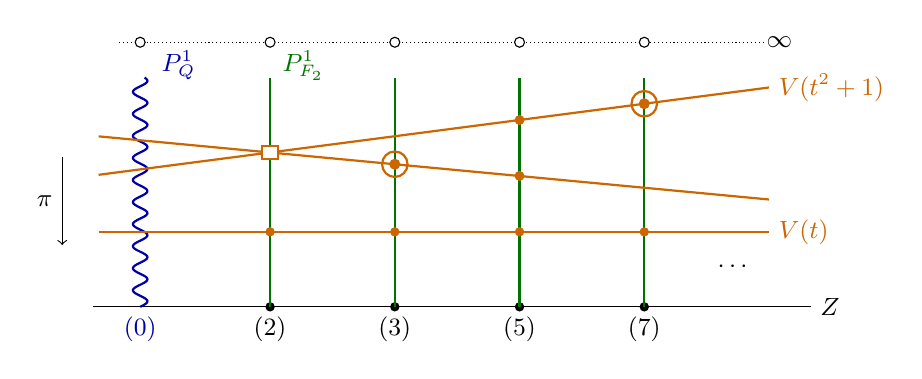
\begin{tikzpicture}[every node/.style={font=\small}, x=1.32cm, y=1.12cm]
\draw (0,0) -- (6.9,0);
\node[right] at (6.9,0) {$\Spec\mathbb Z$};
\foreach \x in {1.7,2.9,4.1,5.3} \fill (\x,0) circle (1.7pt);
\node[below] at (0.45,0) {\textcolor{blue!65!black}{$(0)$}};
\node[below] at (1.7,0) {$(2)$};
\node[below] at (2.9,0) {$(3)$};
\node[below] at (4.1,0) {$(5)$};
\node[below] at (5.3,0) {$(7)$};
\foreach \x in {1.7,2.9,4.1,5.3} \draw[green!45!black, thick] (\x,0) -- (\x,2.6);
\draw[blue!65!black, thick, domain=0:2.6, samples=200] plot ({0.45+0.07*sin(1440*\x)}, \x);
\draw[densely dotted] (0.25,3.0) -- (6.45,3.0);
\foreach \x in {0.45,1.7,2.9,4.1,5.3} \draw[fill=white] (\x,3.0) circle (1.8pt);
\node at (6.6,3.0) {$\infty$};
\node[blue!65!black] at (0.82,2.74) {$\mathbb P^1_{\mathbb Q}$};
\node[green!45!black] at (2.02,2.74) {$\mathbb P^1_{\mathbb F_2}$};
\draw[orange!80!black, thick] (0.05,0.85) -- (6.5,0.85);
\node[orange!80!black, right] at (6.5,0.85) {$V(t)$};
\foreach \x in {1.7,2.9,4.1,5.3} \fill[orange!80!black] (\x,0.85) circle (1.7pt);
\draw[orange!80!black, thick] (0.05,1.497) -- (6.5,2.487);
\draw[orange!80!black, thick] (0.05,1.933) -- (6.5,1.217);
\node[orange!80!black, right] at (6.5,2.487) {$V(t^2+1)$};
\draw[fill=white, draw=orange!80!black, thick] (1.7,1.75) +(-0.075,-0.075) rectangle +(0.075,0.075);
\fill[orange!80!black] (2.9,1.617) circle (2pt);
\draw[orange!80!black, thick] (2.9,1.617) circle (4.6pt);
\fill[orange!80!black] (4.1,2.118) circle (1.8pt);
\fill[orange!80!black] (4.1,1.484) circle (1.8pt);
\fill[orange!80!black] (5.3,2.303) circle (2pt);
\draw[orange!80!black, thick] (5.3,2.303) circle (4.6pt);
\node at (6.15,0.45) {$\cdots$};
\draw[->] (-0.3,1.7) -- (-0.3,0.7) node[midway,left] {$\pi$};
\end{tikzpicture}
\caption{Las fibras de \(\mathbb P^1_{\mathbb Z}\). Cada vertical es la fibra \(\mathbb A^1_{\mathbb F_p}\), y con su punto al infinito es la fibra \(\mathbb P^1_{\mathbb F_p}\) de \(\mathbb P^1_{\mathbb Z}\). La ondulada es la fibra genérica. La sección \(V(t)\) corta cada vertical en el punto racional \(t=0\), y la curva \(V(t^2+1)\) la corta en su fibra: un punto doble sobre \((2)\), dos puntos sobre \((5)\) y un punto de grado \(2\) sobre \((3)\) y \((7)\).}
\label{fig:s11-fibras-proyectiva-z}
\end{figure}

\emph{Qué buscamos.} Una familia integral sobre \(\Spec\mathbb Z\) cuyas fibras sobre los primos que dividen a \(m\) tienen nilpotentes.

\begin{ejem}[La familia \(T_1T_2^2=m\)]
\label{ejem:s11-familia-nilpotentes}
Sea \(m\) un entero no nulo, \(R=\mathbb Z[T_1,T_2]/(T_1T_2^2-m)\), \(X=\Spec R\) y \(f\colon X\to\Spec\mathbb Z\) el morfismo que induce \(\mathbb Z\to R\).
\begin{enumerate}[label=(\roman*)]
\item Si \(p\) es un primo que no divide a \(m\), la fibra sobre \((p)\) es \(\Spec\mathbb F_p[T_1,T_2]/(T_1T_2^2-\bar m)\), isomorfa a \(\Spec\mathbb F_p[T,T^{-1}]\), y es integral. La fibra genérica es \(\Spec\mathbb Q[T_1,T_2]/(T_1T_2^2-m)\), isomorfa a \(\Spec\mathbb Q[T,T^{-1}]\).
\item Si \(p\) divide a \(m\), la fibra sobre \((p)\) es \(\Spec\mathbb F_p[T_1,T_2]/(T_1T_2^2)\). Su espacio es la unión de los cerrados \(V(T_1)\) y \(V(T_2)\), ninguno dentro del otro, y su anillo tiene el nilpotente no nulo \(T_1T_2\).
\item El anillo \(R\) es un dominio, así que \(X\) es integral.
\end{enumerate}
\emph{[Liu, ejemplo 3.1.19, p.~84.]}
\end{ejem}

\emph{Idea.} Si \(c\ne0\), la clase de \(T_2\) es una unidad de \(k[T_1,T_2]/(T_1T_2^2-c)\), con inverso \(c^{-1}T_1T_2\), y \(T_1=cT_2^{-2}\) queda determinada por \(T_2\).

\begin{proof}
Para (i), por la \cref{prop:s11-fibra-afines} y el \cref{ejem:s11-cambio-base-ecuaciones} con \(A=\mathbb Z\), las fibras son las del enunciado, porque \(\kappa((p))=\mathbb F_p\) y \(\kappa((0))=\mathbb Q\), y \(\bar m\ne0\) en \(\mathbb F_p\) cuando \(p\nmid m\). Sea \(k\) un cuerpo y \(c\in k\) no nulo. El homomorfismo \(\theta\colon k[T_1,T_2]\to k[T,T^{-1}]\) con \(T_1\mapsto cT^{-2}\) y \(T_2\mapsto T\) manda \(T_1T_2^2-c\) a \(0\) y da \(\bar\theta\) en el cociente, suprayectivo porque su imagen contiene a \(T\) y a \(T^{-1}=\theta(c^{-1}T_1T_2)\). En el cociente, \(\bar T_2\cdot c^{-1}\bar T_1\bar T_2=c^{-1}\bar T_1\bar T_2^2=1\), y la propiedad universal de la localización, \cref{prop:s11-universales}(b), da \(\psi\colon k[T,T^{-1}]\to k[T_1,T_2]/(T_1T_2^2-c)\) con \(\psi(T)=\bar T_2\). Entonces \(\psi(\bar\theta(\bar T_2))=\bar T_2\) y \(\psi(\bar\theta(\bar T_1))=c(c^{-1}\bar T_1\bar T_2)^2=c^{-1}\bar T_1(\bar T_1\bar T_2^2)=\bar T_1\). Así \(\psi\circ\bar\theta\) es la identidad, porque coincide con ella en los generadores, \(\bar\theta\) es un isomorfismo, y \(k[T,T^{-1}]\subseteq k(T)\) es un dominio. Las dos fibras son integrales por la \cref{defi:s11-integral}. Con \(k=\mathbb F_p\) y \(c=\bar m\) sale la fibra sobre \((p)\), y con \(k=\mathbb Q\) y \(c=m\) la genérica.

Para (ii), si \(p\mid m\), entonces \(\bar m=0\). Por la \cref{prop:s11-topologia-cociente}(a), el espacio de la fibra es el cerrado \(V(T_1T_2^2)\) de \(\Spec\mathbb F_p[T_1,T_2]\). Un primo que contiene a \(T_1T_2^2\) contiene a \(T_1\) o a \(T_2\), así que \(V(T_1T_2^2)=V(T_1)\cup V(T_2)\), con \((T_1)\in V(T_1)\setminus V(T_2)\) y \((T_2)\in V(T_2)\setminus V(T_1)\). El elemento \(T_1T_2\) no es múltiplo de \(T_1T_2^2\), por su grado en \(T_2\), y \((T_1T_2)^2=T_1\cdot T_1T_2^2\) sí lo es.

Para (iii), como polinomio en \(T_1\) con coeficientes en el dominio de factorización única \(\mathbb Z[T_2]\), \(T_2^2T_1-m\) es de grado \(1\) y sus coeficientes \(T_2^2\) y \(-m\) solo tienen las unidades \(\pm1\) como divisores comunes. Por el lema de Gauss, \cref{prop:s08-gauss}, con \(\mathbb Z[T_2]\) en lugar de \(\mathbb Z\) (Lang, \emph{Algebra}, cap.~IV, \S2), es irreducible en \(\mathbb Z[T_2][T_1]\), que es un dominio de factorización única, y por eso es primo.
\end{proof}

Liu llama \emph{degeneración} a este fenómeno: el esquema total \(X\) es integral y sus fibras sobre los primos que dividen a \(m\) tienen nilpotentes.

\subsection{Lectura. Lo que se hizo a mano es la fibra}

Se lee fuera de clase. Junta el \cref{teo:s11-espacio-fibra} con lo que la 8d y la 9b calcularon a mano.

\begin{obs}[Lo que se hizo a mano es la fibra]
\label{obs:s11-mano-es-fibra}
\begin{enumerate}[label=(\alph*)]
\item La 8d dio, para un anillo \(A\) y un primo \(\mathfrak p\), una biyección entre los primos de \(A[t]\) que contraen a \(\mathfrak p\) y los primos de \(\kappa(\mathfrak p)[t]\), y con ella una entre \(\pi^{-1}(\mathfrak p)\) y los puntos de \(\mathbb P^1_{\kappa(\mathfrak p)}\), con \(\pi\colon\mathbb P^1_A\to\Spec A\); véanse \cref{lema:s08-fibra-recta-afin,prop:s08-fibras-proyectiva}. Es el caso afín del \cref{teo:s11-espacio-fibra} con \(B=A[t]\), y sus dos movimientos, localizar en \(A\setminus\mathfrak p\) y reducir módulo \(\mathfrak p\), son los del \cref{lema:s11-localizar-cocientar}. Hoy esa biyección es la proyección de la fibra, es un homeomorfismo, y la fibra es el \(\kappa(\mathfrak p)\)-esquema \(\mathbb P^1_{\kappa(\mathfrak p)}\), por la \cref{obs:s11-cambio-base-proyectiva}.
\item La 9b vio que, sobre un anillo de valoración discreta \(A\) con uniformizante \(\varpi\), los primos de una \(A\)-álgebra \(B\) que contraen a \((0)\) forman \(D(\varpi)\), homeomorfo a \(\Spec B[\varpi^{-1}]\), y los que contraen a \(\mathfrak m=(\varpi)\) forman \(V(\varpi)\), homeomorfo a \(\Spec B/\mathfrak mB\); véase \cref{prop:s09-primos-sobre-dvr}. Es el \cref{teo:s11-espacio-fibra} sobre un anillo de valoración discreta. La fibra genérica es \(\Spec(B\otimes_AK)\cong\Spec B[\varpi^{-1}]\) y la fibra especial es \(\Spec(B\otimes_A\kappa)\cong\Spec B/\mathfrak mB\), por la \cref{prop:s11-fibra-afines}, porque todo \(a\ne0\) de \(A\) es una unidad por una potencia de \(\varpi\), y por eso invertir los \(\varphi(a)\) con \(a\ne0\) es invertir \(\varphi(\varpi)\).
\item La tabla de los primos de \(\mathbb Z[i]\) sobre cada \((p)\) de la 9b, \cref{ejem:s11-enteros-gaussianos}, es la lista de las fibras cerradas de \(\Spec\mathbb Z[i]\to\Spec\mathbb Z\) del \cref{ejem:s11-fibras-gaussianos}.
\end{enumerate}
\emph{[Sesiones 8d y 9b. Liu, prop.~3.1.16 y ejemplo 3.1.18.]}
\end{obs}

\section{Lemas y afirmaciones de hoy}
\label{sec:s11-lemas-hoy}

Los cinco enunciados siguientes son los argumentos que completa el grupo, y tres de ellos forman parte de la tarea final del curso. La unicidad del producto fibrado, \cref{lema:s11-unicidad-producto}, es el argumento de la Tarea 1, ejercicio 1.3.A. Los esbozos de los tres primeros están en la lectura de las secciones anteriores; los dos últimos se completan sin esbozo.

\begin{ejer}[Primero de la tarea final]
\label{ejer:s11-restrccion-abiertos}
Demuestra la \cref{afirm:s11-restrccion-abiertos}: si \((P,\mathrm{pr}_X,\mathrm{pr}_Y)\) es un producto fibrado de \(X\to S\) y \(Y\to S\) y \(U\subseteq X\) es abierto, entonces \(\mathrm{pr}_X^{-1}(U)\) es un producto fibrado de \(U\to S\) y \(Y\to S\), y en particular \(U\times_XY\cong f^{-1}(U)\) para todo morfismo \(f\colon Y\to X\).

\emph{Pista.} Aplica la propiedad universal de \(P\) al par \((j_U\circ a,b)\) y comprueba que la imagen del morfismo obtenido está en \(\mathrm{pr}_X^{-1}(U)\), para factorizarlo por el \cref{lema:s11-imagen-abierto}. Para el caso particular, usa que \(X\times_XY\cong Y\).
\end{ejer}

\begin{ejer}[Segundo de la tarea final]
\label{ejer:s11-polinomios-tensorial}
Demuestra el \cref{lema:s11-polinomios-tensorial}: el homomorfismo \(\lambda\) de \(A[x_1,\ldots,x_n]\otimes_AB\) en \(B[x_1,\ldots,x_n]\) que lleva \(G\otimes b\) a \(bG^\varphi\) es un isomorfismo de anillos, y por eso \(\mathbb A_A^n\times_{\Spec A}\Spec B\cong\mathbb A_B^n\).

\emph{Pista.} Comprueba que \(B[x_1,\ldots,x_n]\), con \(G\mapsto G^\varphi\) y la inclusión de \(B\), cumple la propiedad universal de la \cref{prop:s11-tensor-algebras}(b). Para la unicidad, usa que \(A[x]\) está generado por \(A\) y las \(x_k\), y aplica la unicidad de la Tarea 1, ejercicio 1.3.A con las flechas al revés.
\end{ejer}

\begin{ejer}[Tercero de la tarea final]
\label{ejer:s11-proyectiva-fp}
Demuestra el \cref{lema:s11-proyectiva-fp}: los \(\Spec\) de las reducciones módulo \(p\) de las cartas se pegan en \(c\colon\mathbb P^1_{\mathbb F_p}\to\mathbb P^1_{\mathbb Z}\), y \((\mathbb P^1_{\mathbb F_p},c,\pi')\) es un producto fibrado de \(\pi\) y \(\sigma\).

\emph{Pista.} Comprueba que las dos reducciones llevan \(s\) a \(t^{-1}\) y que coinciden en \(D(t)=D(s)\), para pegarlas con el \cref{lema:s11-morfismos-pegan}. En cada carta usa el \cref{lema:s11-polinomios-tensorial} con \(n=1\) y la \cref{afirm:s11-restrccion-abiertos}, y para la unicidad, la del producto sobre \(U_0\cap U_1\).
\end{ejer}

\begin{ejer}
\label{ejer:s11-localizar-cocientar}
Demuestra el \cref{lema:s11-localizar-cocientar}: \(B\otimes_A\kappa(\mathfrak p)\cong B_{\mathfrak p}/\mathfrak pB_{\mathfrak p}\), y \(b\mapsto b\otimes1\) es la localización seguida del cociente.

\emph{Pista.} Escribe \(\kappa(\mathfrak p)\cong A_{\mathfrak p}\otimes_A A/\mathfrak p\) y asocia. Usa \(B\otimes_AA_{\mathfrak p}\cong B_{\mathfrak p}\), y para el cociente el isomorfismo \(M\otimes_A(A/I)\cong M/IM\) de la \cref{prop:s11-tensor-cociente-localizacion}(b). Identifica después la imagen de \(b\otimes1\).
\end{ejer}

\begin{ejer}
\label{ejer:s11-contraer-p}
Demuestra la \cref{afirm:s11-contraer-p}: si \(\varphi^{-1}(\mathfrak q)\subseteq\mathfrak p\), entonces \(\mathfrak q\) no corta a \(\varphi(A\setminus\mathfrak p)\), el ideal \(\mathfrak qB_{\mathfrak p}\) es primo, y contiene a \(\mathfrak pB_{\mathfrak p}\) si y solo si \(\varphi^{-1}(\mathfrak q)=\mathfrak p\).

\emph{Pista.} Para la primalidad, usa la correspondencia de la \cref{prop:s11-primos-localizacion}. Para la contención, compara las contracciones a \(A\) de \(\mathfrak qB_{\mathfrak p}\) y de \(\mathfrak pB_{\mathfrak p}\), que son \(\varphi^{-1}(\mathfrak q)\) y \(\mathfrak p\).
\end{ejer}
